%  LaTeX support: latex@mdpi.com 
%  For support, please attach all files needed for compiling as well as the log file, and specify your operating system, LaTeX version, and LaTeX editor.

%=================================================================
\documentclass[toxics,article,submit,pdftex,moreauthors]{Definitions/mdpi} 
%\documentclass[preprints,article,submit,pdftex,moreauthors]{Definitions/mdpi} 
% For posting an early version of this manuscript as a preprint, you may use "preprints" as the journal. Changing "submit" to "accept" before posting will remove line numbers.

% Below journals will use APA reference format:
% admsci, behavsci, businesses, econometrics, economies, education, ejihpe, games, humans, ijfs, journalmedia, jrfm, languages, psycholint, publications, tourismhosp, youth

% Below journals will use Chicago reference format:
% arts, genealogy, histories, humanities, jintelligence, laws, literature, religions, risks, socsci

%--------------------
% Class Options:
%--------------------

%---------
% article
%---------
% The default type of manuscript is "article", but can be replaced by: 
% abstract, addendum, article, benchmark, book, bookreview, briefcommunication, briefreport, casereport, changes, clinicopathologicalchallenge, comment, commentary, communication, conceptpaper, conferenceproceedings, correction, conferencereport, creative, datadescriptor, discussion, entry, expressionofconcern, extendedabstract, editorial, essay, erratum, fieldguide, hypothesis, interestingimages, letter, meetingreport, monograph, newbookreceived, obituary, opinion, proceedingpaper, projectreport, reply, retraction, review, perspective, protocol, shortnote, studyprotocol, supfile, systematicreview, technicalnote, viewpoint, guidelines, registeredreport, tutorial,  giantsinurology, urologyaroundtheworld
% supfile = supplementary materials

%----------
% submit
%----------
% The class option "submit" will be changed to "accept" by the Editorial Office when the paper is accepted. This will only make changes to the frontpage (e.g., the logo of the journal will get visible), the headings, and the copyright information. Also, line numbering will be removed. Journal info and pagination for accepted papers will also be assigned by the Editorial Office.

%---------
% pdftex
%---------
% The option pdftex is for use with pdfLaTeX. Remove "pdftex" for (1) compiling with LaTeX & dvi2pdf (if eps figures are used) or for (2) compiling with XeLaTeX.

%=================================================================
% MDPI internal commands - do not modify
\firstpage{1} 
\makeatletter 
\setcounter{page}{\@firstpage} 
\makeatother
\pubvolume{1}
\issuenum{1}
\articlenumber{0}
\pubyear{2025}
\copyrightyear{2025}
%\externaleditor{Firstname Lastname} % More than 1 editor, please add `` and '' before the last editor name
\datereceived{ } 
\daterevised{ } % Comment out if no revised date
\dateaccepted{ } 
\datepublished{ } 
%\datecorrected{} % For corrected papers: "Corrected: XXX" date in the original paper.
%\dateretracted{} % For retracted papers: "Retracted: XXX" date in the original paper.
\hreflink{https://doi.org/} % If needed use \linebreak
%\doinum{}
%\pdfoutput=1 % Uncommented for upload to arXiv.org
%\CorrStatement{yes}  % For updates
%\longauthorlist{yes} % For many authors that exceed the left citation part

%=================================================================
% Add packages and commands here. The following packages are loaded in our class file: fontenc, inputenc, calc, indentfirst, fancyhdr, graphicx, epstopdf, lastpage, ifthen, float, amsmath, amssymb, lineno, setspace, enumitem, mathpazo, booktabs, titlesec, etoolbox, tabto, xcolor, colortbl, soul, multirow, microtype, tikz, totcount, changepage, attrib, upgreek, array, tabularx, pbox, ragged2e, tocloft, marginnote, marginfix, enotez, amsthm, natbib, hyperref, cleveref, scrextend, url, geometry, newfloat, caption, draftwatermark, seqsplit
% cleveref: load \crefname definitions after \begin{document}

%=================================================================
% Please use the following mathematics environments: Theorem, Lemma, Corollary, Proposition, Characterization, Property, Problem, Example, ExamplesandDefinitions, Hypothesis, Remark, Definition, Notation, Assumption
%% For proofs, please use the proof environment (the amsthm package is loaded by the MDPI class).

%=================================================================
% Full title of the paper (Capitalized)
\Title{Biomonitoring-Based Risk Assessment of Pyrethroid Exposure in the U.S.
using High-Throughput and Physiologically Based Kinetic Models} 

% MDPI internal command: Title for citation in the left column
\TitleCitation{Biomonitoring-Based Risk Assessment of Pyrethroid Exposure in
the U.S. using High-Throughput and Physiologically Based Kinetic Models}

% Author Orchid ID: enter ID or remove command
\newcommand{\orcidauthorA}{0000-0003-0163-2766} 
%\newcommand{\orcidauthorB}{0000-0000-0000-000X} % Add \orcidB{} behind the author's name

% Authors, for the paper (add full first names)
\Author{Nan-Hung Hsieh*\orcidA{} and Eric S. Kwok}

%\longauthorlist{yes}

% MDPI internal command: Authors, for metadata in PDF
\AuthorNames{Nan-Hung Hsieh and Eric S.C. Kwok}

% MDPI internal command: Authors, for citation in the left column, only choose below one of them according to the journal style
% If this is a Chicago style journal 
% (arts, genealogy, histories, humanities, jintelligence, laws, literature, religions, risks, socsci): 
% Lastname, Firstname, Firstname Lastname, and Firstname Lastname.

% If this is a APA style journal 
% (admsci, behavsci, businesses, econometrics, economies, education, ejihpe, games, humans, ijfs, journalmedia, jrfm, languages, psycholint, publications, tourismhosp, youth): 
% Lastname, F., Lastname, F., \& Lastname, F.

% If this is a ACS style journal (Except for the above Chicago and APA journals, all others are in the ACS format): 
% Lastname, F.; Lastname, F.; Lastname, F.

\AuthorCitation{Hsieh, N.-H.; Kwok, S.E.}

% Affiliations / Addresses (Add [1] after \address if there is only one affiliation.)
\address[1]{Human Exposure \& Health Effects Modeling Section, Human Health
Assessment Branch, Department of Pesticide Regulation, California Environmental
Protection Agency, Sacramento, CA, USA; \\ }

% Contact information of the corresponding author
%\corres{Correspondence: e-mail@e-mail.com; Tel.: (optional; include country code; if there are multiple corresponding authors, add author initials) +xx-xxxx-xxx-xxxx (F.L.)}
\corres{Correspondence: \href{mailto:nan-hung.hsieh@cdpr.ca.gov}{\nolinkurl{nan-hung.hsieh@cdpr.ca.gov}}}

% Current address and/or shared authorship
%\firstnote{Current address: Affiliation.}  % Current address should not be the same as any items in the Affiliation section.
%\secondnote{These authors contributed equally to this work.}
% The commands \thirdnote{} till \eighthnote{} are available for further notes

%\simplesumm{} % Simple summary

%\conference{} % An extended version of a conference paper

% Abstract (Do not insert blank lines, i.e. \\) 
\abstract{Pyrethroid insecticides have been extensively utilized in
agriculture and residential areas in the United States. We attempt to
evaluate its exposure risk in populations by age using available
biomonitoring data. We analyzed pyrethroid metabolite concentrations in
urine using the National Health and Nutrition Examination Survey
(NHANES) data. Reverse dosimetry was conducted with a high-throughput
model and a physiologically based kinetic (PBK) model integrated with a
Bayesian inference framework. We further derive Benchmark Dose (BMD)
values and systematic points of departure in rats using Bayesian BMD and
PBK models. Margins of exposure (MOE) were calculated to evaluate
neurotoxic risk based on estimated daily oral intake and dose metrics in
plasma and brain. Results from both models showed higher pyrethroid
exposure in young children compared to other age groups. All estimated
risk values were within acceptable level of acute neurotoxic effect.
Additionally, MOEs calculated from oral doses were lower than those
derived from internal doses, highlighting that traditional external
exposure assessments tend to overestimate risk compared to advanced
internal dose-based techniques. In conclusion, combining high-throughput
and PBK approaches enhances the understanding of human health risks
associated with pyrethroid exposures, underscoring their potential for
future applications in following tracking and health risk assessment.}

% Keywords
\keyword{Reverse dosimetry; Bayeisan; Pyrethroids; Urinary metabolites,
Exposure risk}

% The fields PACS, MSC, and JEL may be left empty or commented out if not applicable
%\PACS{J0101}
%\MSC{}
%\JEL{}

%%%%%%%%%%%%%%%%%%%%%%%%%%%%%%%%%%%%%%%%%%
% Only for the journal Diversity
%\LSID{\url{http://}}

%%%%%%%%%%%%%%%%%%%%%%%%%%%%%%%%%%%%%%%%%%
% Only for the journal Applied Sciences
%\featuredapplication{Authors are encouraged to provide a concise description of the specific application or a potential application of the work. This section is not mandatory.}
%%%%%%%%%%%%%%%%%%%%%%%%%%%%%%%%%%%%%%%%%%

%%%%%%%%%%%%%%%%%%%%%%%%%%%%%%%%%%%%%%%%%%
% Only for the journal Data
%\dataset{DOI number or link to the deposited data set if the data set is published separately. If the data set shall be published as a supplement to this paper, this field will be filled by the journal editors. In this case, please submit the data set as a supplement.}
%\datasetlicense{License under which the data set is made available (CC0, CC-BY, CC-BY-SA, CC-BY-NC, etc.)}

%%%%%%%%%%%%%%%%%%%%%%%%%%%%%%%%%%%%%%%%%%
% Only for the journal Toxins
%\keycontribution{The breakthroughs or highlights of the manuscript. Authors can write one or two sentences to describe the most important part of the paper.}

%%%%%%%%%%%%%%%%%%%%%%%%%%%%%%%%%%%%%%%%%%
% Only for the journal Encyclopedia
%\encyclopediadef{For entry manuscripts only: please provide a brief overview of the entry title instead of an abstract.}

%%%%%%%%%%%%%%%%%%%%%%%%%%%%%%%%%%%%%%%%%%
% Only for the journal Advances in Respiratory Medicine, Smart Cities and Sensors
%\addhighlights{yes}
%\renewcommand{\addhighlights}{%

%\noindent This is an obligatory section in “Advances in Respiratory Medicine'' and ``Smart Cities”, whose goal is to increase the discoverability and readability of the article via search engines and other scholars. Highlights should not be a copy of the abstract, but a simple text allowing the reader to quickly and simplified find out what the article is about and what can be cited from it. Each of these parts should be devoted up to 2~bullet points.\vspace{3pt}\\
%\textbf{What are the main findings?}
% \begin{itemize}[labelsep=2.5mm,topsep=-3pt]
% \item First bullet.
% \item Second bullet.
% \end{itemize}\vspace{3pt}
%\textbf{What is the implication of the main finding?}
% \begin{itemize}[labelsep=2.5mm,topsep=-3pt]
% \item First bullet.
% \item Second bullet.
% \end{itemize}
%}

%%%%%%%%%%%%%%%%%%%%%%%%%%%%%%%%%%%%%%%%%%
\begin{document}

%%%%%%%%%%%%%%%%%%%%%%%%%%%%%%%%%%%%%%%%%%
\section{Introduction}\label{introduction}

Pyrethroids, synthetic insecticides prevalent in residential and
agricultural pest control, have raised health concerns due to their extensive
use and potential adverse effects \citep{burns2018pyrethroid}. Their usage has
significantly increased in recent decades both in the United States and
globally. Mounting evidence suggest that exposure to pyrethroids are linked to
adverse health effects, including diabetes, neurotoxicity, and cardiovascular
disease. Consequently, scientists and researchers have actively monitored and
reconstructed pyrethroid exposure among residential and occupational
populations \citep{zartarian2012quantifying, bravo2022occupational}.

Various exposure tools have been developed to estimate both aggregate
and cumulative exposure doses of current-use pesticides, including
pyrethroids
\citep{tulve2011methodologies, zartarian2012quantifying, xue2014epa}. In
earlier research, \citet{tulve2011methodologies} applied three methodologies
developed by the United States Environmental Protection Agency (U.S. EPA),
including The Standard Operating Procedures for Residential Pesticide Exposure
Assessment \citep{us2012standard}, Draft Protocol for Measuring Children's
Non-Occupational Exposure to Pesticides by all Relevant Pathways
\citep{us2001draft}, and the Stochastic Human Exposure and Dose Simulation
(SHEDS) Model for Multimedia, Multipathway Pollutants, to estimate cumulative
residential exposures to pyrethroids for children aged 4-6 years. Among these
approaches, the SHEDS framework was initially developed to estimate children's
residential exposure and dose to chlorpyrifos via dermal contact and
non-dietary ingestion \citep{zartarian2000modeling} and has been applied to
several metals, polychlorinated biphenyls, and pyrethroids for regulatory
decisions \citep{tulve2011methodologies, xue2015modeling,
zartarian2017children}. For pyrethroids, \citet{zartarian2012quantifying} used
permethrin as a benchmark to verify the performance of exposure prediction
models, such as the physiologically based kinetic (PBK) model
\citep{tornero2012pharmacokinetic} and the SHEDS high-throughput model
\citep{isaacs2014sheds}, due to the abundance of experimental exposure and
toxicokinetic (TK) data.

Biomonitoring is widely recognized as a reliable method for quantifying
human exposure to pyrethroids in populations
\citep{barr2010urinary, quindroit2021estimating, tarazona2022tiered}. It
captures aggregate exposure across all pathways and is an essential tool
for chemical risk assessment
\citep{blount2007perchlorate, sobus2015uses}. Health-based guidance
values derived from biomonitoring data provide effective and
comprehensible evaluations of pyrethroid exposure potential
\citep{apel2023human}. Biomarkers commonly used to estimate population
exposure include urinary metabolites such as 3-phenoxybenzoic acid
(3PBA), 4-fluoro-3-phenoxybenzoic acid (FPBA),
3-(2,2-dibromovinyl)-2,2-dimethylcyclopropane carboxylic acid (DBCA),
and
cis-/trans-3-(2,2-dichlorovinyl)-2,2-dimethylcyclopropane-1-carboxylic
acid (DCCA). These biomarkers can either be linked to specific
pyrethroid parent compounds or shared among multiple pyrethroids. For
example, FPBA and DBCA are specific to cyfluthrin and deltamethrin,
respectively, while 3PBA is a general metabolite of several pyrethroids,
exhibiting lower toxicity compared to the parent compounds.
Biomonitoring data in the U.S. population, extensively tracked by the
National Health and Nutrition Examination Survey (NHANES) over decades,
indicate that children may experience higher pyrethroid exposures than
adolescents and adults \citep{barr2010urinary}. However, biomonitoring
data alone have limitations in exposure assessment due to factors such
as variable exposure frequency, sampling time, and inter-individual
variability \citep{aylward2017variation}.

Despite the limitations, biomonitoring data can be used with
computational exposure modeling tools in exposure reconstruction. TK
modeling is an example that utilizes ``reverse-dosimetry'' approach to
estimate the exposure profile of chemicals
\citep{egeghy2011assessment, lin2023reconstructing} based on the
observed levels of chemical in human body. The U.S. EPA's ExpoCast
project developed a comprehensive high-throughput approach in the
Systematic Empirical Evaluation of Models (SEEM) framework to
effectively predict the population exposure for chemical prioritization
\citep{wambaugh2013high, stanfield2022bayesian}. The SEEM framework was
used to predict the daily intake based on NHANES biomonitoring data with
Bayesian statistical approach. It is worth noting that the outcomes from
the prediction were used to compare with other high-throughput
approaches, such as SHEDS \citep{isaacs2014sheds} and the consensus
model with multiple forward exposure model predictions
\citep{ring2018consensus}.

To better predict chemical intake, physiologically based kinetic (PBK) models
have been applied in several research studies \citep{tan2006use, allen2007use,
lyons2008computational, tornero2012pharmacokinetic, moreau2017using}. This
sophisticated modeling approach considers absorption, distribution, metabolism,
and elimination processes in the body. Compared to the U.S. EPA's
high-throughput approach, which is based on generic TK model and that assumes
steady-state equilibrium with mass balance (100\% absorption) to simplified
model structure, PBK models provide more accurate parameter estimations and
have been validated with experimental TK data. A study conducted by the U.S.
EPA reported that ``The SEEM approach evaluates predictors of exposure based on
how well they correlate with estimates of chemical intake rate from
biomonitoring'' \citep{ring2018consensus}. Thus, the reliability of chemical
intake rates inferred from biomonitoring data is crucial for determining model
performance. It is essential to examine the biomonitoring data quality and its
representativeness alongside model parameters. Given the various prediction
tools developed, each with strengths and uncertainties in exposure prediction,
integrating information from different tools can strengthen the scientific
rigor of the exposure assessment process \citep{moreau2017using}.

The primary purpose of this study was to understand and track the
exposure and dosimetry conditions of pyrethroids in the U.S. population
based on available biomonitoring data and assess human health risks.
This study employs an open-sourced and well-developed pyrethroid PBK
model to estimate the exposure of pyrethroids and their isomers
(deltamethrin, cis- and trans-isomers of permethrin, cypermethrin, and
cyfluthrin). The U.S. EPA's high-throughput model outputs were compared
with the PBK model predictions, as both reverse dosimetry approaches use
the same biomonitoring data (cis- and trans-DCCA, 3PBA, F-PBA, and DBCA)
from NHANES. Using multiple biomarkers reduces uncertainties regarding
the representation of systemic exposures to the agent
\citep{lin2023reconstructing}. These comparisons offer insights into
establishing criteria for accurate exposure prediction in biomonitoring
data-driven exposure assessments.


%%%%%%%%%%%%%%%%%%%%%%%%%%%%%%%%%%%%%%%%%%

\section{Materials and Methods}\label{materials-and-methods}

\subsection{Problem definition}\label{problem-definition}

Figure \ref{fig1} illustrates the concept of the study approach. Several
uncertainties that may impact the current modeling process and their solutions
were addressed as follows:

\begin{itemize}
\item
  \textbf{Model Specification:} The uncertainty of model specification
  was addressed by comparing estimations using two reverse dosimetry
  modeling approaches. Estimates from other available resources (e.g.,
  official databases, publications) were incorporated for exposure
  comparison.
\item
  \textbf{Linkage of Pyrethroids and Metabolites:} Five downstream
  metabolites are associated with four upstream pyrethroid exposures.
  The pyrethroid PBK model quantified the fraction of metabolites formed
  by a parent compound by calibrated model parameter through human TK
  data \citep{quindroit2019estimating}. The high-throughput approach
  also addresses the stoichiometric fraction of transformation between
  multiple parents and their metabolites.
\item
  \textbf{Non-detect Values Below the Limit of Detection (LOD):}
  Nondetect values below the LOD introduce uncertainty in exposure
  estimation. Bayesian inference with the PBK model was used to predict
  these non-detect values. The high-throughput method assumes that
  population urine concentrations are log-normally distributed across
  all compounds, allowing non-detect values to be imputed through the
  geometric mean and standard deviation of the simulated distribution.
\item
  \textbf{Short Half-Lives of Pyrethroids and Metabolites:} Pyrethroids
  and their metabolites typically have short half-lives less than 24
  hours \citep{hays2007biomonitoring}, meaning their concentrations
  change rapidly over a short period. This study used NHANES spot urine
  samples as surrogates for 24-hour average urinary concentrations,
  which may underestimate the daily dose rate due to random sampling
  times relative to exposure events \citep{aylward_interpreting_2012}.
  Under the same daily exposure dose but with different dosing time
  intervals, biomonitoring using spot urine samples and 24-hour averages
  can vary widely. Urinary half-lives in humans of approximately 12
  hours have been measured for several pyrethroids following oral
  exposures \citep{leng1997biological, woollen_metabolism_1992}. Kinetic
  simulations indicate that once-daily exposures lead to within-day
  peaks in urinary concentration approximately two- to three-fold higher
  than the steady-state average concentration for compounds with a
  half-life of 12 hours \citep{aylward_screening_level_2018}.
  Additionally, factors such as hydration status, creatinine excretion
  rate, and metabolism patterns can impact concentrations by a factor of
  2 to 3 \citep{scher2007agreement}. The exposure difference from urine
  concentration to exposure was addressed by quantifying the variation
  in observed data and intake prediction.
\end{itemize}

\begin{figure}[H]
\centering
\begin{adjustwidth}{-4cm}{}
\centering
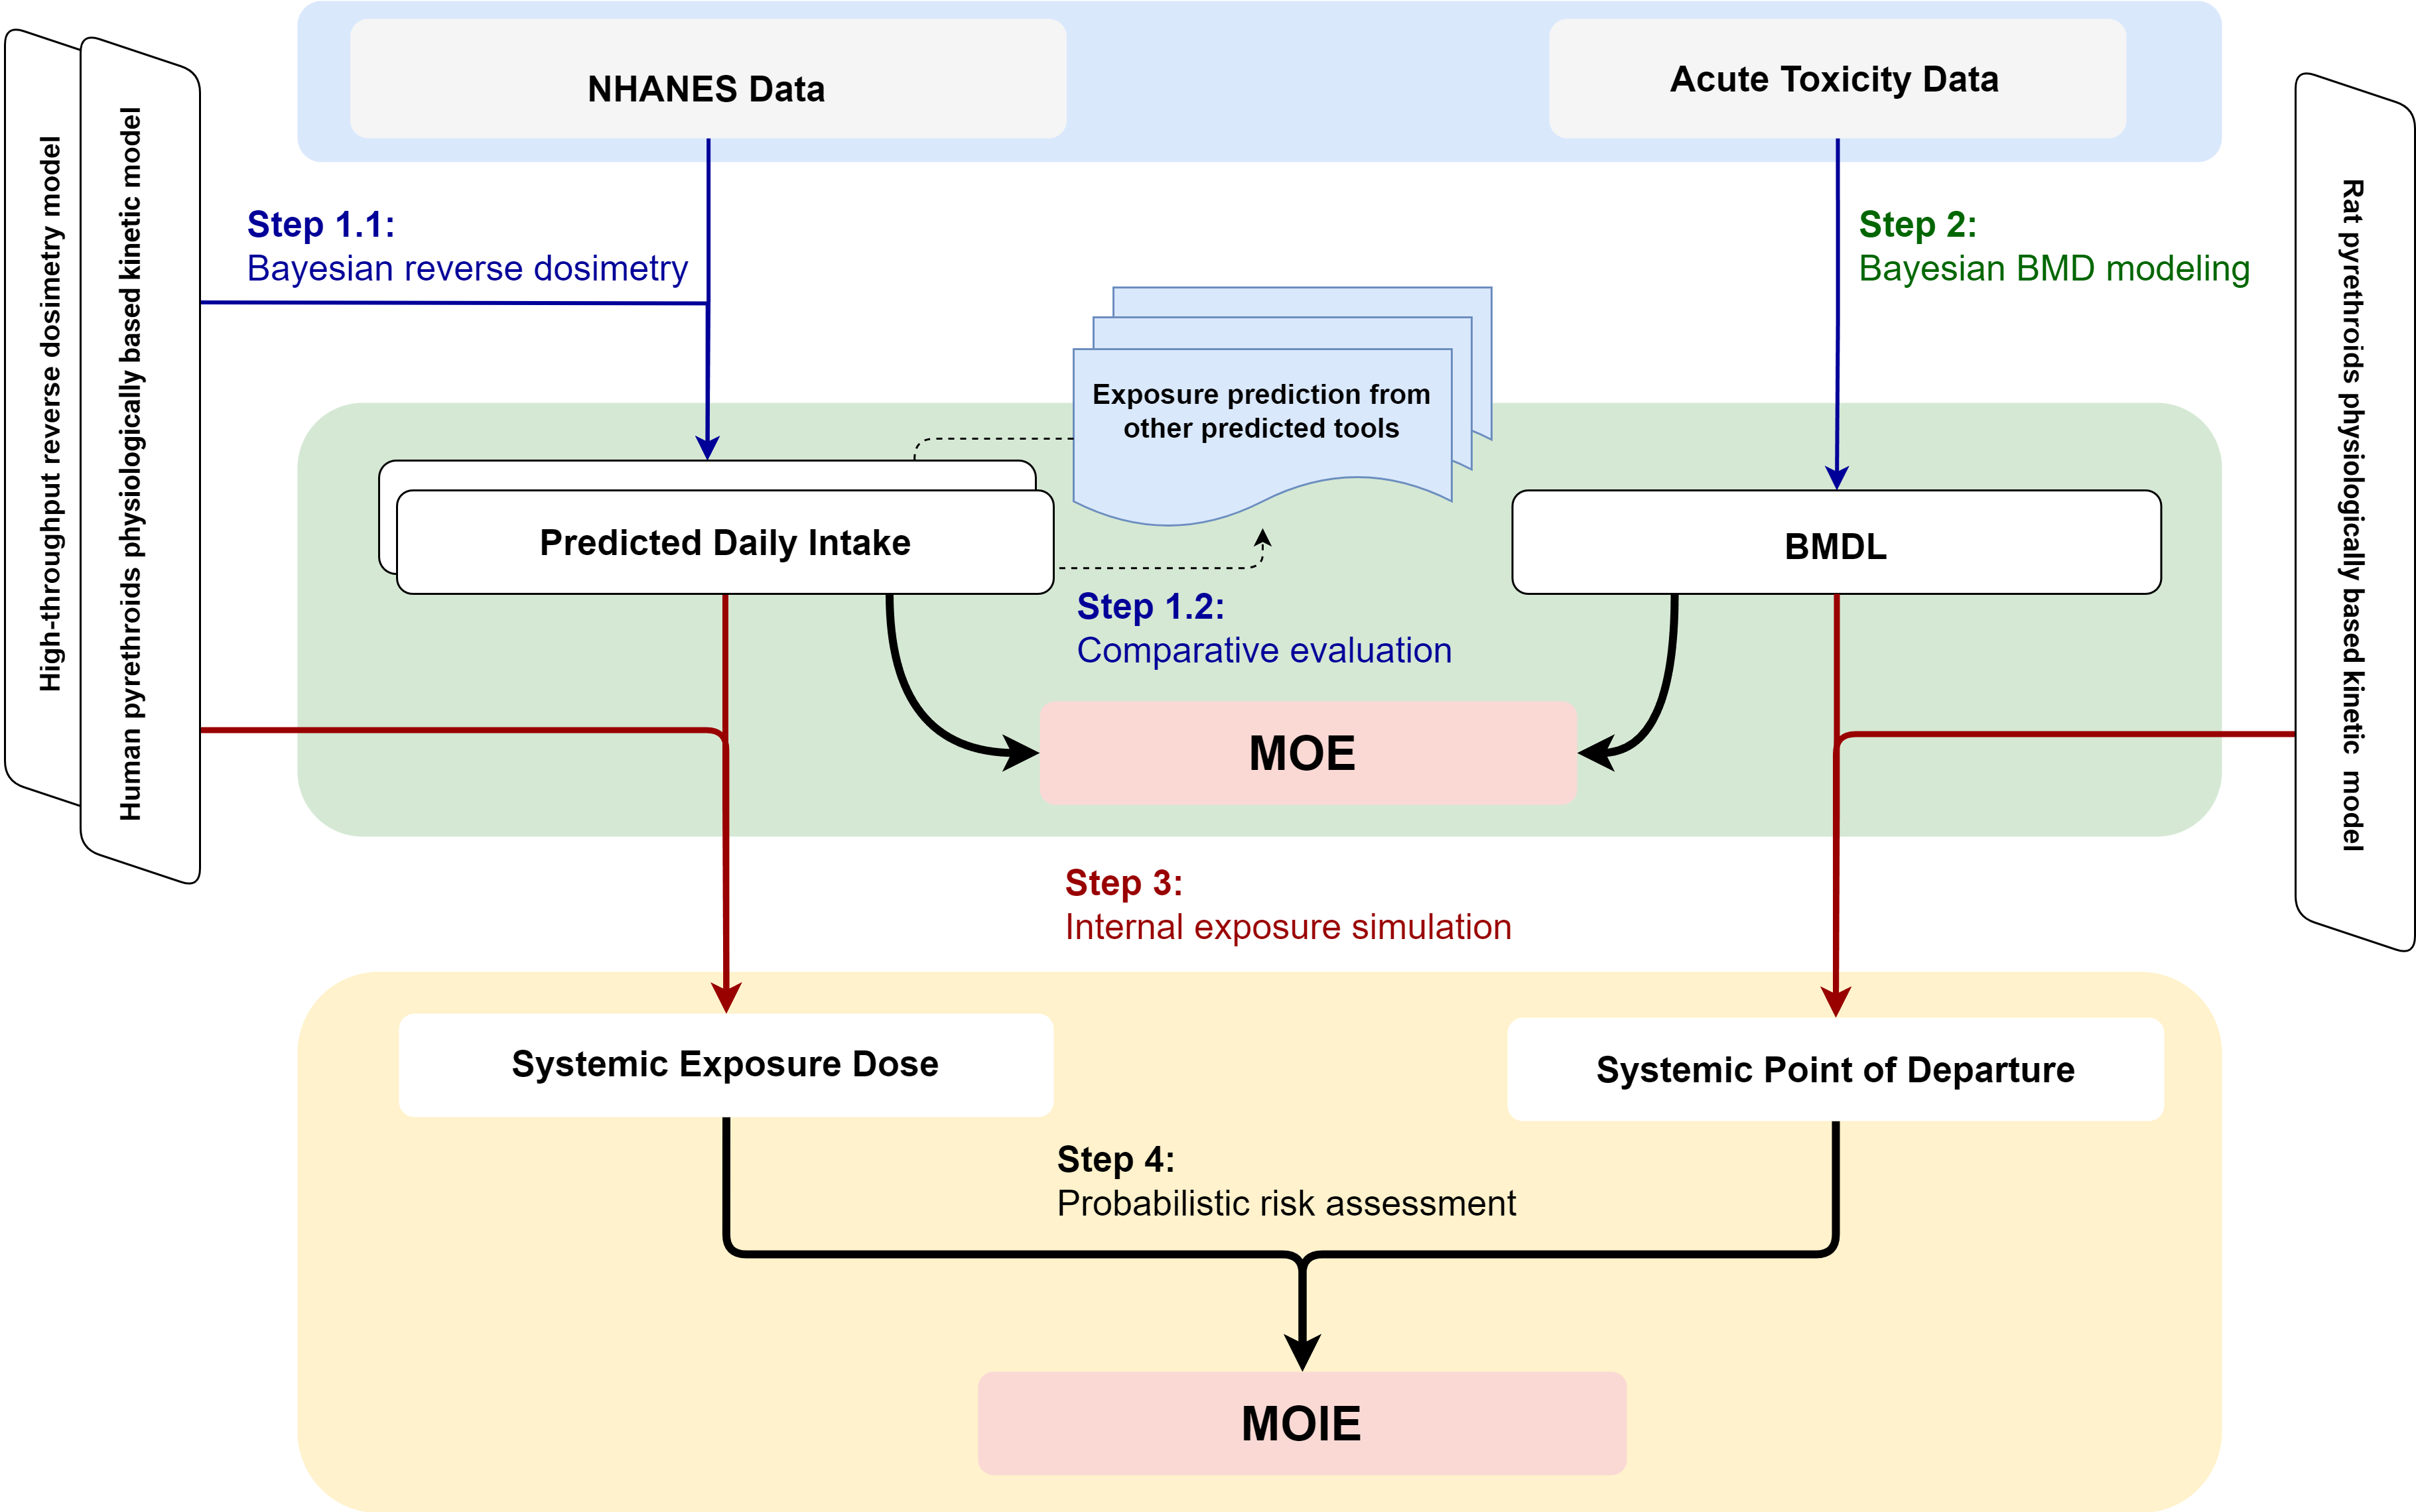
\includegraphics[width=\linewidth]{figures/fig1.drawio}
\hfill
\end{adjustwidth}
\caption{Schematic diagram of the overall study workflow. The study consists of 
four key steps: (1) using Bayesian reverse dosimetry to estimate daily intake from 
National Health and Nutrition Examination Survey biomonitoring data, (2) applying 
the Bayesian benchmark dose approach to reanalyze dose-response data from animal 
neurotoxicity studies, (3) simulating systemic exposure dose and determining the 
point of departure based on external daily intake and benchmark dose thresholds, 
and (4) probabilistically estimating the margin of internal exposure by integrating 
predicted exposure levels with effect thresholds. Note: BMD, Benchmark Dose; BMDL, Benchmark Dose Lower Confidence Limit; MOE, Margin of Exposure; MOIE, Margin of Internal Exposure; NHANES, National Health and Nutrition Examination Survey.\label{fig1}}
\end{figure}


\subsection{NHANES biomonitoring data}\label{nhanes-biomonitoring-data}

We utilized the NHANES database for exposure reconstruction. Data
collection began with the biennial cycle spanning 1999-2001, covering
the general U.S. population aged six years and older. Seven subsequent
cycles were conducted to investigate pyrethroid exposure. Notably, only
the 1999-2000 and 2001-2002 cycles conducted comprehensive surveys of
five metabolites (cis- and trans-DCCA, 3PBA, FPBA, and DBCA). Over time,
the metabolites cis-DCCA and DBCA were gradually phased out from the
survey, with their last inclusion noted in the 2007-2008 and 2010-2011
cycles, respectively. Detailed information about the metabolites
measured by NHANES in each cycle are founded in Table \ref{tab:taba1}.
It is worth noting that the LODs were not consistent across cycles.

\subsection{The physiologically based kinetic
model}\label{the-physiologically-based-kinetic-model}

A generic PBK model, previously developed by the Council for the
Advancement of Pyrethroid Human Risk Assessment
\citep{song2019evaluation, mallick2020development, mallick_physiologically_2020},
was used to describe the TK of pyrethroids in humans. This model was
derived and validated using time-course data from rats
\citep{mirfazaelian_development_2006, tornero2010evaluation}. We
extended the PBK model to verify the human time-concentration profile of
metabolites in urine (Figure \ref{fig:fig2}). The structure was based on
the generic model for pyrethroids, with the addition of the inhalation
exposure route as described by \citet{beaudouin2010stochastic} and
\citet{quindroit2019estimating}. To validate the refined PBK model,
human TK data were adopted from published studies, including exposure
routes of oral intake, dermal contact, and inhalation
\citep{leng1997human, leng1997biological, ratelle2015toxicokinetics, ratelle2015time}.
Throughout the metabolic process, four parent compounds were observed to
transform into seven metabolites (Table \ref{tab:taba2}).

\begin{figure}[H]
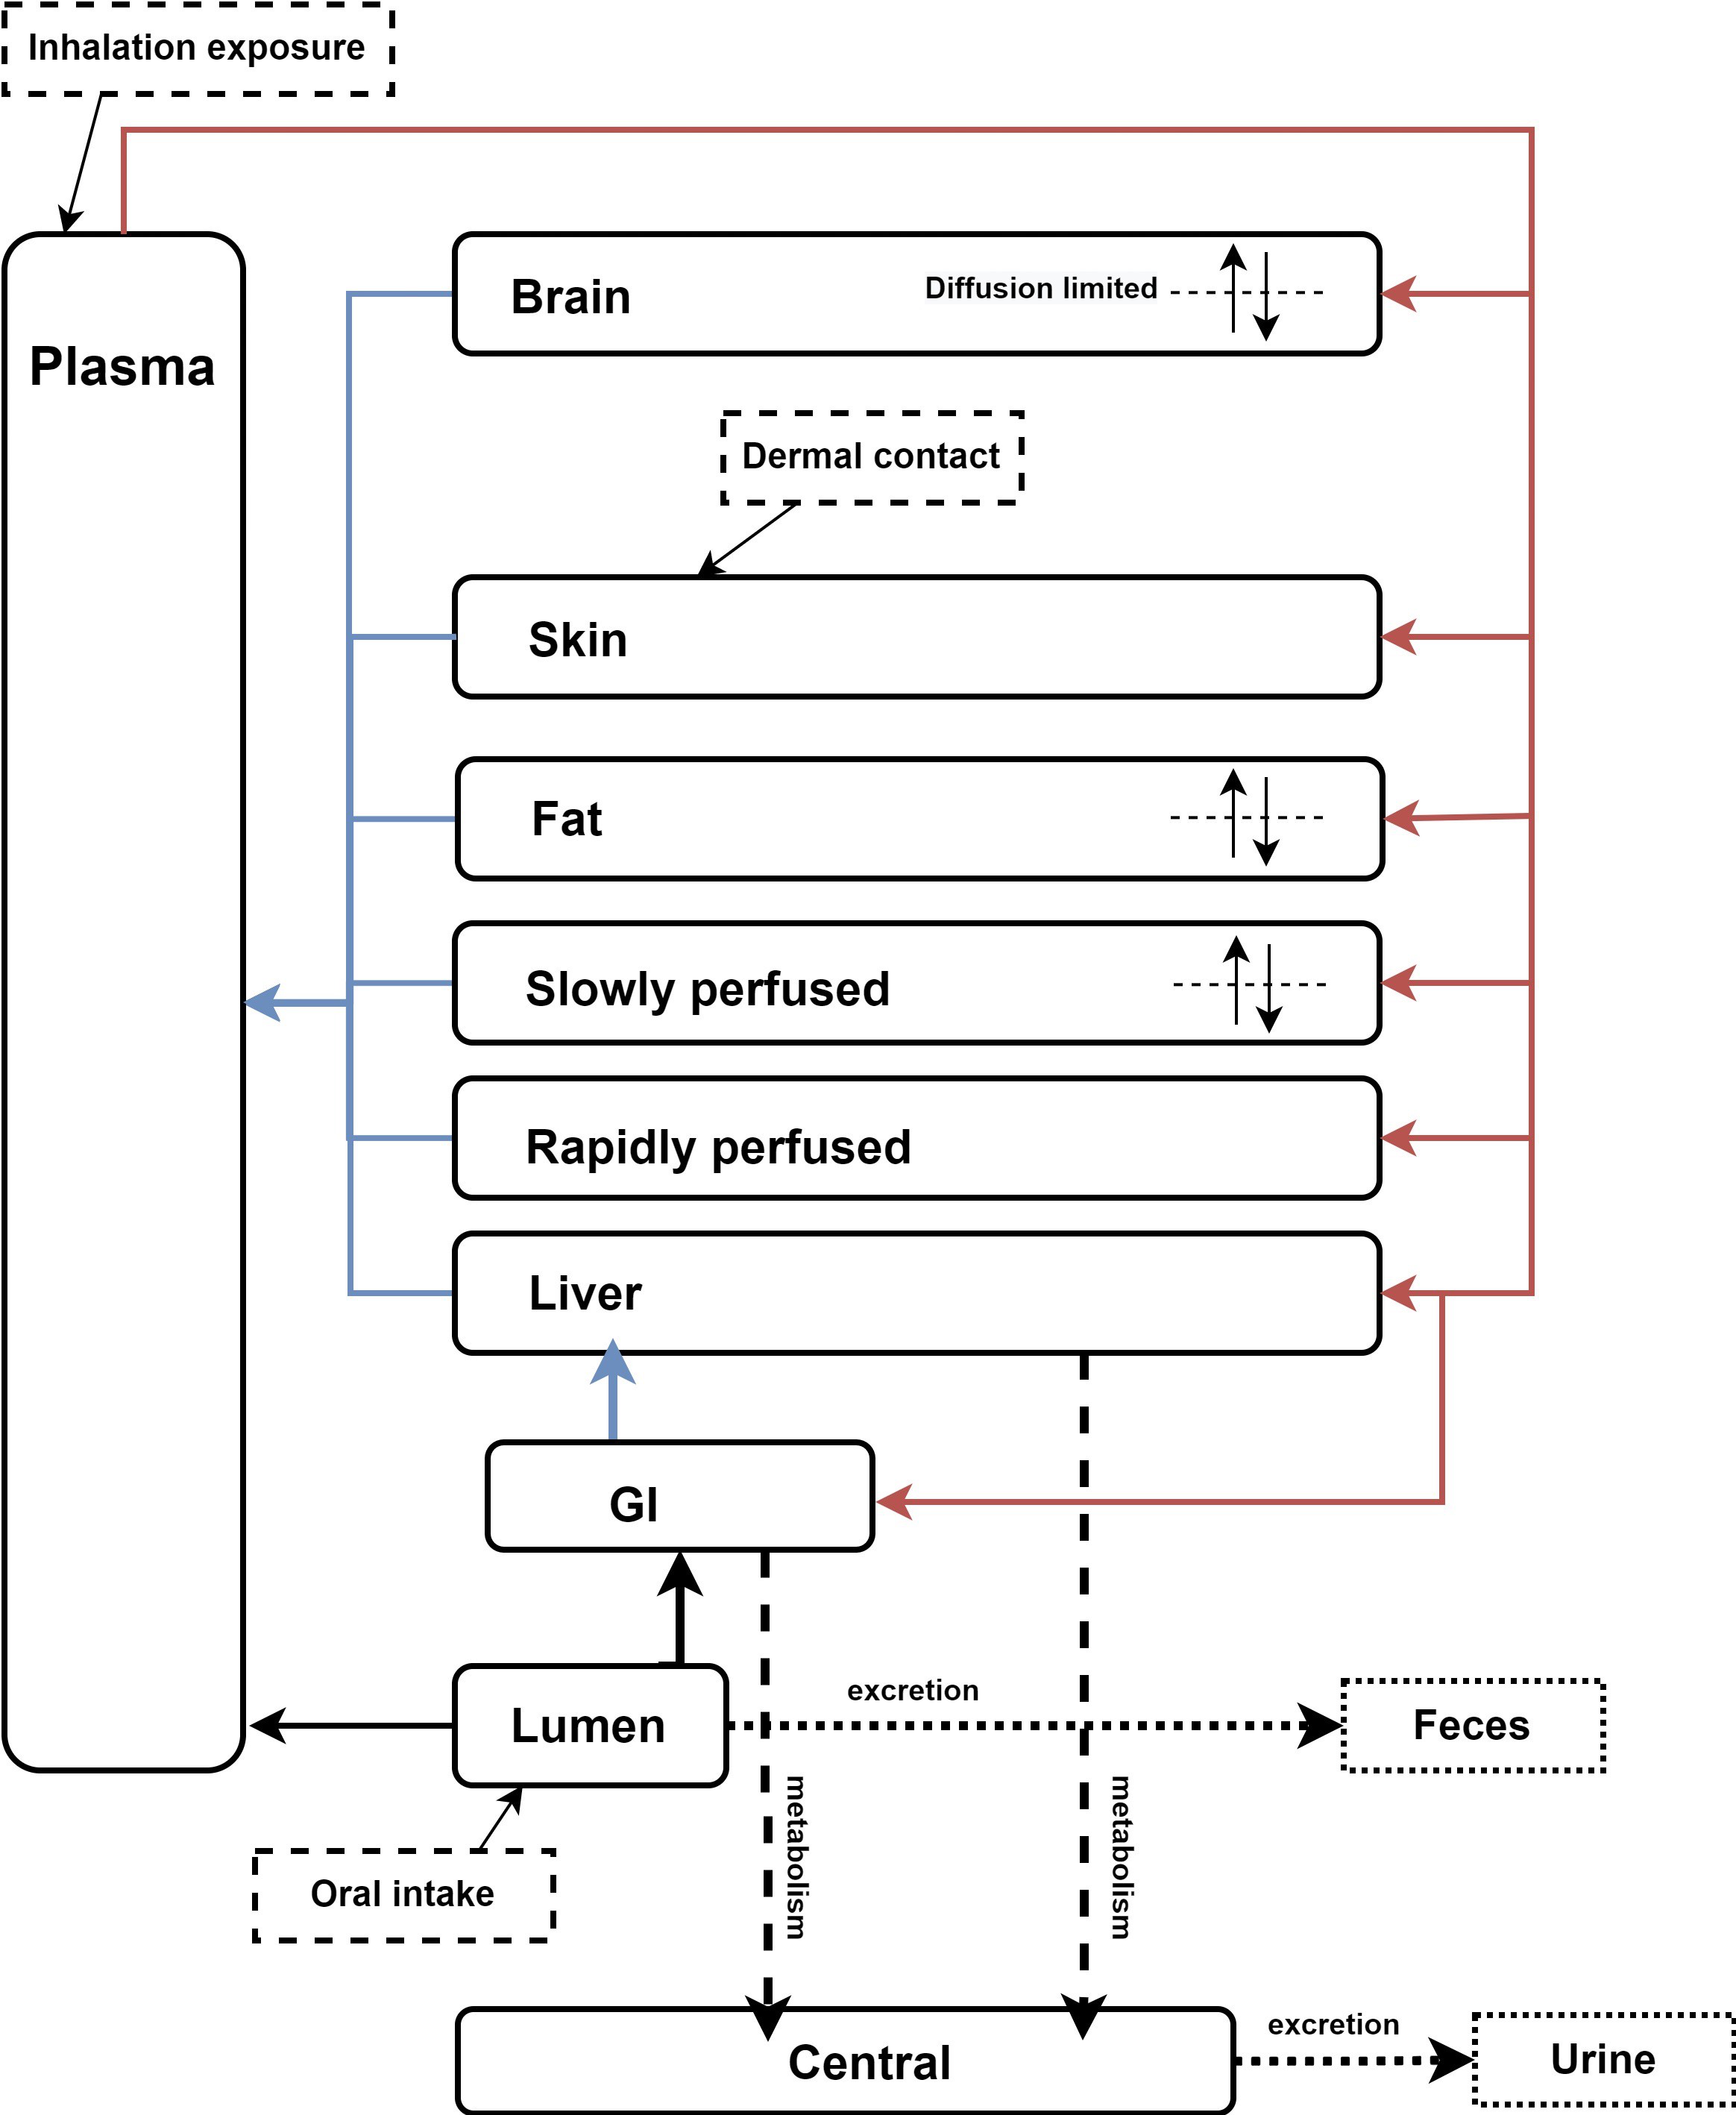
\includegraphics[width=0.8\linewidth,]{figures/fig2} \caption{Refined generic physiologically based kinetic (PBK) model for pyrethroids and their metabolites. The diagram illustrates the PBK model structure, depicting the absorption, distribution, metabolism, and elimination processes of pyrethroids and their metabolites in the human body.}\label{fig:fig2}
\end{figure}

As the examined data were spot urine samples without information on the
time between exposure and sampling, we assumed all observations were
under steady-state exposure conditions. Meaning each observation
reflects the daily average exposure. Consequently, we employed an
analytical solution for the PBK model to simplify the estimation of the
relationship between intake dose rate and metabolite urine
concentration. Under steady-state conditions, only a few parameters are
expected to significantly affect metabolite concentration. The
description of the critical parameters relevant to urine concentration,
along with their corresponding values used in the PBK model are found in
the Table \ref{tab:taba3}. Specifically, physiological parameters such
as body weight, urine creatinine, and daily creatinine were found to be
associated with urine concentration, while factors such as blood flow
and organ weight were not considered impactful. Additionally,
chemical-specific parameters, including the rate constants of oral
absorption and fecal elimination are also directly related to
metabolites urine concentration.

\subsection{Bayesian population
modeling}\label{bayesian-population-modeling}

Bayesian population modeling was adopted to predict population exposure
to pyrethroids in residential scenarios across all age groups
\citep{allen2007use, lyons2008computational}. By applying Bayes' rule,
the posterior probability of daily pyrethroid intake was estimated based
on the measured urinary metabolite concentrations. The prior
distribution of daily intake was calculated with urinary metabolite
concentration treated as likelihood. A uniform (non-informative)
distribution of each exposure concentration was assigned in the interval
from \(10^{-12}\) to \(10^0\). An inverse gamma distribution was used to
describe the prior distribution of population variance
\citep{lyons2008computational}, with scale and shape parameters equal to
2.25 and 5.0, respectively, assuming both the coefficient of uncertainty
and variability in the prior distribution are equal to 2.

For observations above the LOD, the likelihood of the data given the
model predictions was assumed to be log-normal, based on the
specification of the variance of the residual error. This variance could
arise from measurement error, intra-individual heterogeneity, and (or)
model misspecification. For observations below the LOD, a normal
distribution with a standard deviation equal to LOD/4 was used to
describe the deviation between the data and the model, with all
observations below the LOD set at 0 and LOD/2, respectively. These
settings aim to provide different inferences for nondetected values
below the LOD and examine the overall goodness-of-fit. The variances for
each of the corresponding residual errors were given half-normal
distributions with a standard deviation of 0.3, corresponding to a
geometric standard deviation of 1.7.

Physiological parameters, such as body weight, were sourced from NHANES.
To reduce computational burden, the chemical specific parameter (e.g.,
transformation fractions and isomeric ratios) were set to fixed values
based on \citet{quindroit2019estimating}. The intake rate ratio between
cypermethrin and permethrin was set by referring to the California
Department of Pesticide Regulation's (DPR) Pesticide Use Reporting
database (\url{https://www.cdpr.ca.gov/docs/pur/purmain.htm}) and
previous results from the high-throughput model
\citep{stanfield2022bayesian}.

\subsection{High-throughput model and other exposure prediction
tools}\label{high-throughput-model-and-other-exposure-prediction-tools}

The U.S. EPA's ExpoCast project provides reliable intake estimates based
on NHANES biomonitoring data \citep{wambaugh2013high}. This approach
uses Bayesian statistical methods to infer the probabilistic exposure of
intake rates for parent chemicals, assuming a log-normal distribution of
product concentrations in NHANES urine samples. The geometric mean and
standard deviation were first calculated and used to estimate
observations below the LOD. These parameters were verified by comparing
the generated cumulative density function (CDF) to the population CDF of
the sample data, including quantiles and confidence limits from NHANES
data. The statistical characteristics of metabolites were then converted
to units of exposure through a reverse dosimetry TK model with a
steady-state assumption. For pyrethroids with multiple metabolites, the
fractions of each metabolite were also calculated.

In addition to the exposure estimates from biomonitoring data, numerous
studies and databases related to pyrethroid exposure and risk assessment
were reviewed to compare and summarize the estimation of exposure doses.
The exposure predictions from the U.S. EPA CompTox Chemicals Dashboard
(\url{https://comptox.epa.gov/dashboard/}) were adopted to compare with
the estimated exposure from the current study. The web-based application
includes predictions of daily chemical exposure based on the results of
EPA's ExpoCast project, and utilizing approaches from Chemical and
Products Database, SEEM, and NHANES exposure inferences
\citep{dionisio2018chemical, wambaugh2022exposure}.

\subsection{Exposure variability}\label{exposure-variability}

The ratio of the 95th and 50th percentiles (P95/P50) was calculated to
assess the variability through the spot urine samples of NHANES
biomonitoring data relative to the daily exposure dose. The analysis was
conducted for metabolites with over 60\% of measurements detected
\citep{faure_evaluation_2020}. According to
\citet{aylward_interpreting_2012}, the variation of observed exposure
dose is similar to the predicted dose and can be used to assess the
misestimation of intake in reverse dosimetry. Based on this concept, we
estimated the underlying daily dose distributions to inform the
interpretation of population biomonitoring data in the context of
uncertainty quantification. The P95/P50 of predicted intake doses were
also calculated and compared with the ratio of biomonitoring measures.
The resulting ratio provides an indication of the degree of over- or
under-prediction of variation in doses as reflected by the variation in
biomarker concentrations.

\section{Bayesian benchmark dose
modeling}\label{bayesian-benchmark-dose-modeling}

This study focuses on acute exposure and risk assessment due to (1) the
spot urine samples from NHANES not being suitable for interpreting
repeated long-term exposure, (2) the short half-lives of pyrethroids
reflecting recent rather than continuous exposure, and (3) the lack of
robust sub-chronic and chronic toxicity data for exposure risk
assessment.

Acute oral toxicity data were sourced from open literature
\citep{wolansky_relative_2006}, as well as from Benchmark dose (BMD)
data analysis conducted by U.S. EPA
(\url{https://www.regulations.gov/document/EPA-HQ-OPP-2008-0331-0064}).
The data were selected because of rigorous data standard required for
federal regulatory purpose. Neurotoxicity was assessed by locomotor
activity. The Bayesian BMD was applied to reanalyze the toxicity data
using a web-based system \citep{shao_kan_web_2018}.

The default models for continuous data and non-informative prior were
used to fit the dose-response data, using Markov chain Monte Carlo
(MCMC) simulation. Three Markov chains were calculated with 30,000
iterations per chain. The model distributions were estimated using the
last half of iterations (15,000 iterations per chain). The model average
from 8 continuous models using the posterior model weights was used to
establish the BMD distribution. One standard deviation of the response
from the control was chosen for BMD as the suggested choice by U.S. EPA.

\subsection{Risk estimates}\label{risk-estimates}

The margin of exposure (MOE) and margin of internal exposure (MOIE)
approaches were used to calculate human health risk, based on the (1)
PBK-estimated daily oral intake and (2) the corresponding internal
exposure dose metrics. The MOE is a quantitative tool used by DPR and
most regulatory agencies to determine the potential risk arising from
exposure to a pesticide and other chemicals
\citep{beaudouin2010stochastic, beauvais_human_2010}. It is defined as
the ratio of the critical point of departure (POD) value derived from
the definitive acute, sub-chronic, or chronic studies to the estimated
human exposure. The resulting value is compared to the acceptable or
target MOE, which values at or above the target MOE are generally
considered protective against the toxicity of compound in question. For
this analysis, MOE was calculated by dividing the BMDL by the exposure
estimate of pyrethroid.

Comparing with MOE, the MOIE is a relatively advanced exposure
assessment strategy that relies on the sophisticated PBK model to
provide the robust evaluation for decision making
\citep{bessems_margin_2017}. Because of the correlation between brain
concentration and acute neurotoxic effects
\citep{scollon_correlation_2011}, this study derived the MOIE by
dividing BMDL-derived dose metrics, such as peak concentration (Cmax)
and area under the curve (AUC) in the plasma and the brain. The rat PBK
model from \citet{song2019evaluation} was applied with the BMDL to
simulate the time-concentration curve based on a single oral intake in
\citet{wolansky_relative_2006}, and to estimate the dose metrics. The
refined life-stage human PBK model was applied with Monte Carlo
simulations, to estimate the distribution of the four dose metrics
according to the estimated daily exposure dose. The parameter settings
for the Monte Carlo simulation are founded in th Table \ref{tab:taba4}.

\subsection{Computational settings and
evaluation}\label{computational-settings-and-evaluation}

The PBK model, along with its input conditions, was developed for use in
the GNU MCSim software (version 6.1.0) \citep{bois_gnu_2009}. All other
statistical analyses and visualizations were conducted using the latest
version of the R programming language (version 4.4.0) with the relevant
packages. Additionally, the U.S.EPA-developed R package bayesmarker
\citep{stanfield2022bayesian} was used to estimate the exposure intake
dose rate based on the high-throughput approach. For both Bayesian
modeling approaches, three independent Markov Chains were run to
estimate the posterior distributions. Convergence was assessed as
recommended by Gelman and Rubin \citep{gelman1992inference}. The
goodness of fit was evaluated by assessing the posterior distribution of
measurement error. All R and GNU MCSim codes for modeling and analyses
will be provided upon request.

%%%%%%%%%%%%%%%%%%%%%%%%%%%%%%%%%%%%%%%%%%
\section{Results}\label{results}

\subsection{Exploratory analysis of the biomonitoring
data}\label{exploratory-analysis-of-the-biomonitoring-data}

The current analysis encompassed a total of 18,665 individuals across
seven biennial cycles from 1999-2000 to 2015-2016. The 2015-2016 cycle
introduced an additional survey focusing on children under six years old
but covering only three metabolites. To facilitate a comparison of
exposure doses with prior research, the population was segmented into
five distinct age groups: \textless6, 6-11, 12-19, 20-65, and
\textgreater65 years. The grouping was same as the U.S. EPA's ExpoCast
project.

Initial analysis of summary statistics revealed notable patterns in
detection rates of various biomonitoring results (Table
\ref{tab:taba5}). The consistently high detection rate of 3PBA was
particularly striking because the detection rate exceed 60\% across all
observed years. Conversely, the detection of DBCA remained consistently
low, consistently registering at less than 2\%. A significant
observation is the trend in FPBA detection, which exhibited a
discernible increase over the last three biennial cycles (2010-2016),
indicating a noteworthy shift in exposure levels over time. Under the
same LOD conditions, the detection rate of 3PBA showed an increasing
trend from around 70\% before 2010 to 95\% in the latest survey
(2015-2016). During the 2007-2016 period, the detection rates of FPBA
and trans-DCCA increased from 6.5\% to 13.2\% and from 15.8\% to 37.5\%,
respectively.

While examining the cumulative distribution of urine concentrations
across different age groups (Figure \ref{fig:figa1}), no significant
disparities were evident. However, a clear upward trend in detection
rates emerged over the same three biennial cycles for 3PBA, suggesting a
potential temporal influence on exposure levels.

\subsection{Model evaluation}\label{model-evaluation}

The refined PBK model performed well with human TK experiments, which
includes 176 data points from 17 TK profiles of 5 pyrethroid
metabolites (Figure \ref{fig:figa2}). Using the default parameter values, 99\% of the predictions
fall within a 10-fold range, approximately 75\% within a 3-fold range,
and 65\% within a 2-fold range of the observed values. The calibrated
PBK model was used to estimate the daily intakes of the four pyrethroid
parent compounds. The observed biomonitoring data was compared with the
corresponding model predictions (Figure \ref{fig:fig3}). Overall, the
refined PBK model performs better during the earlier biennial cycles
(1999-2000 and 2001-2002), where all five metabolites were fully
investigated.

\begin{figure}[H]
\centering
\begin{adjustwidth}{-2cm}{}
\centering
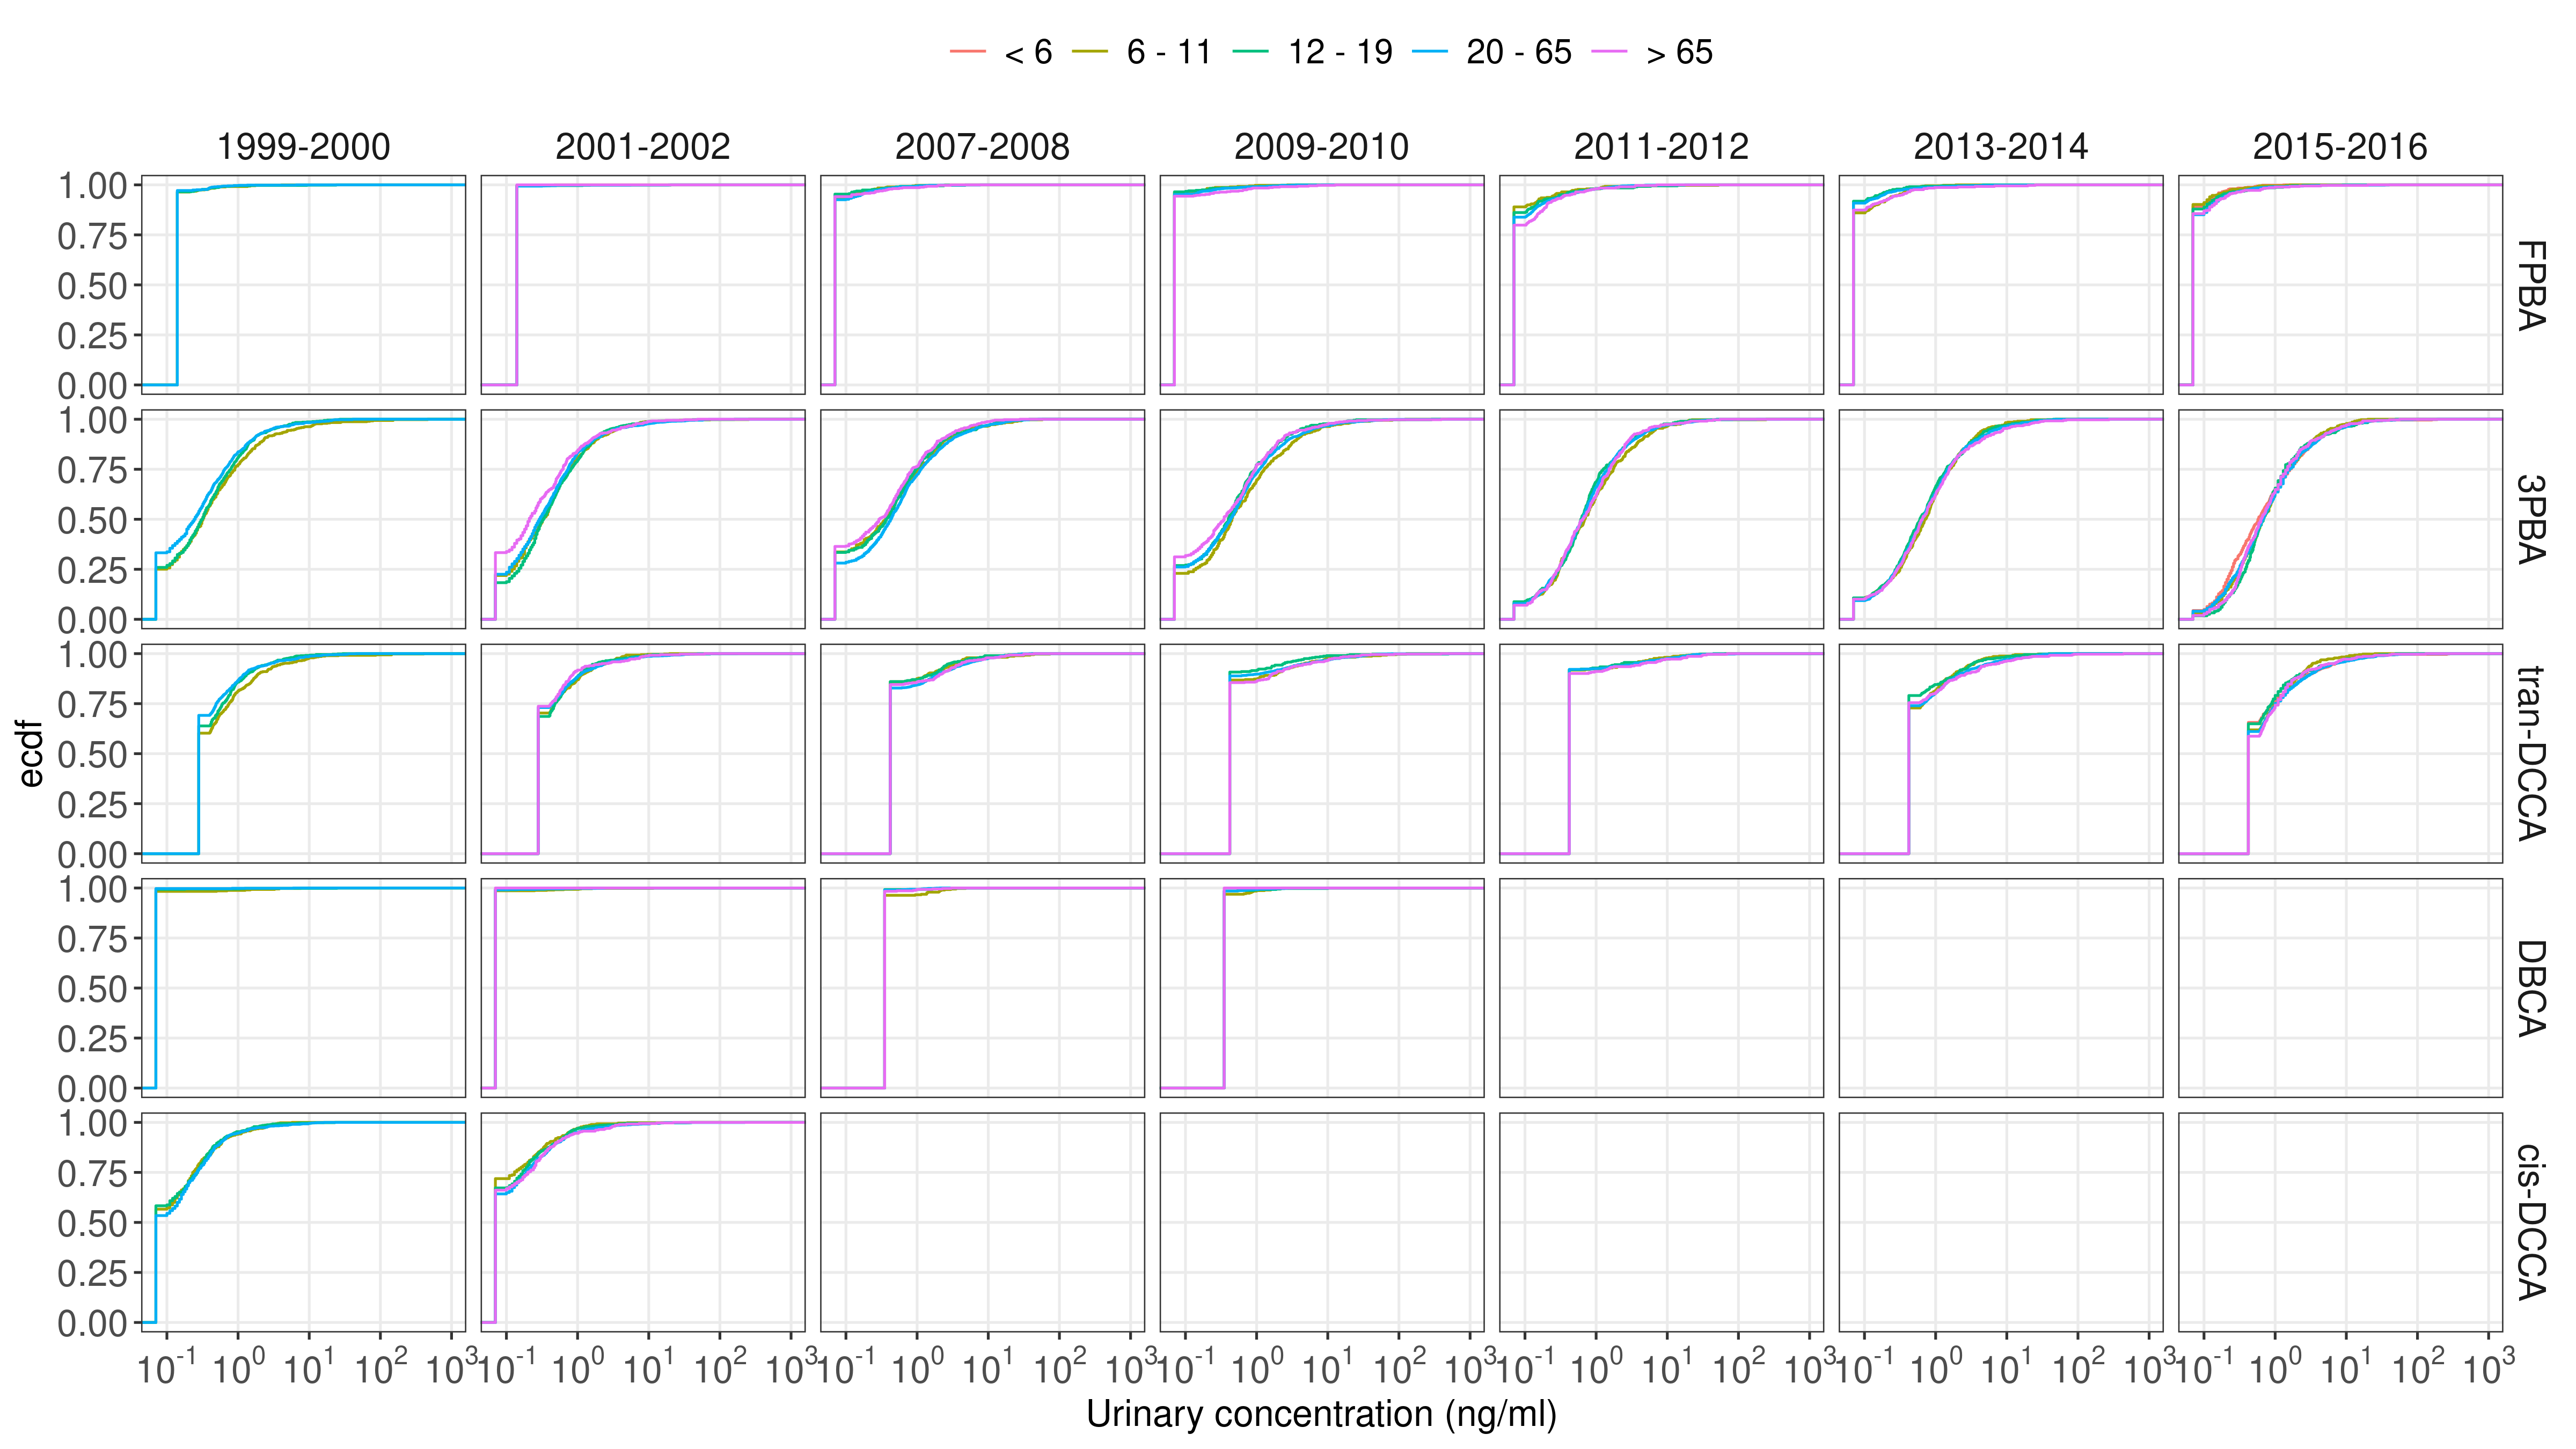
\includegraphics[width=\linewidth]{figures/fig3}
\hfill
\end{adjustwidth}
\caption{Goodness-of-fit evaluation for the total population across NHANES
cycles. These plots compare observed and predicted urinary concentrations of
pyrethroid metabolites for the total population across NHANES cycles.
Predictions are based on parameters from the final Markov Chain Monte Carlo
iterations. The solid line represents a perfect match between observed and
predicted values, while dashed lines indicate error margins within a ten-fold
difference.\label{fig:fig3}}
\end{figure}

Figure \ref{fig:fig4} demonstrates an overall comparison of model
predictions from the PBK and high-throughput models. It is commonly
observed that the PBK model yields higher intake rate estimates compared
to high-throughput approaches. For example, in the 2013-2014 cycle, the
median geometric mean intake rates for cyfluthrin, cypermethrin, and
permethrin were estimated to be \(1.02 \times
10^{-5}\), \(5.31 \times 10^{-6}\), and \(5.31 \times 10^{-5}\) mg/kg-d,
respectively, for the 6-11 age group using the PBK model. In contrast,
the high-throughput approach estimated the median population exposure
for cyfluthrin, cypermethrin, and permethrin to be
\(9.37 \times 10^{-7}\), \(1.54
\times 10^{-6}\), and \(1.49 \times 10^{-6}\) mg/kg-d, respectively,
which is lower than the PBK predictions. Moreover, the PBK model
encountered difficulty in estimating the intake rate of deltamethrin
during the latest three biennial cycles (2010-2016) due to the absence
of DBCA data. Analysis of the estimated geometric mean intake rates
reveals that permethrin and cypermethrin exhibit greater consistency
between the two methods, with over 70\% of estimates differing by less
than a tenfold margin. Conversely, cyfluthrin and deltamethrin display
larger disparities, with 43\% and 64\%, respectively, exceeding this
threshold.

\begin{figure}[H]
\centering
\centering
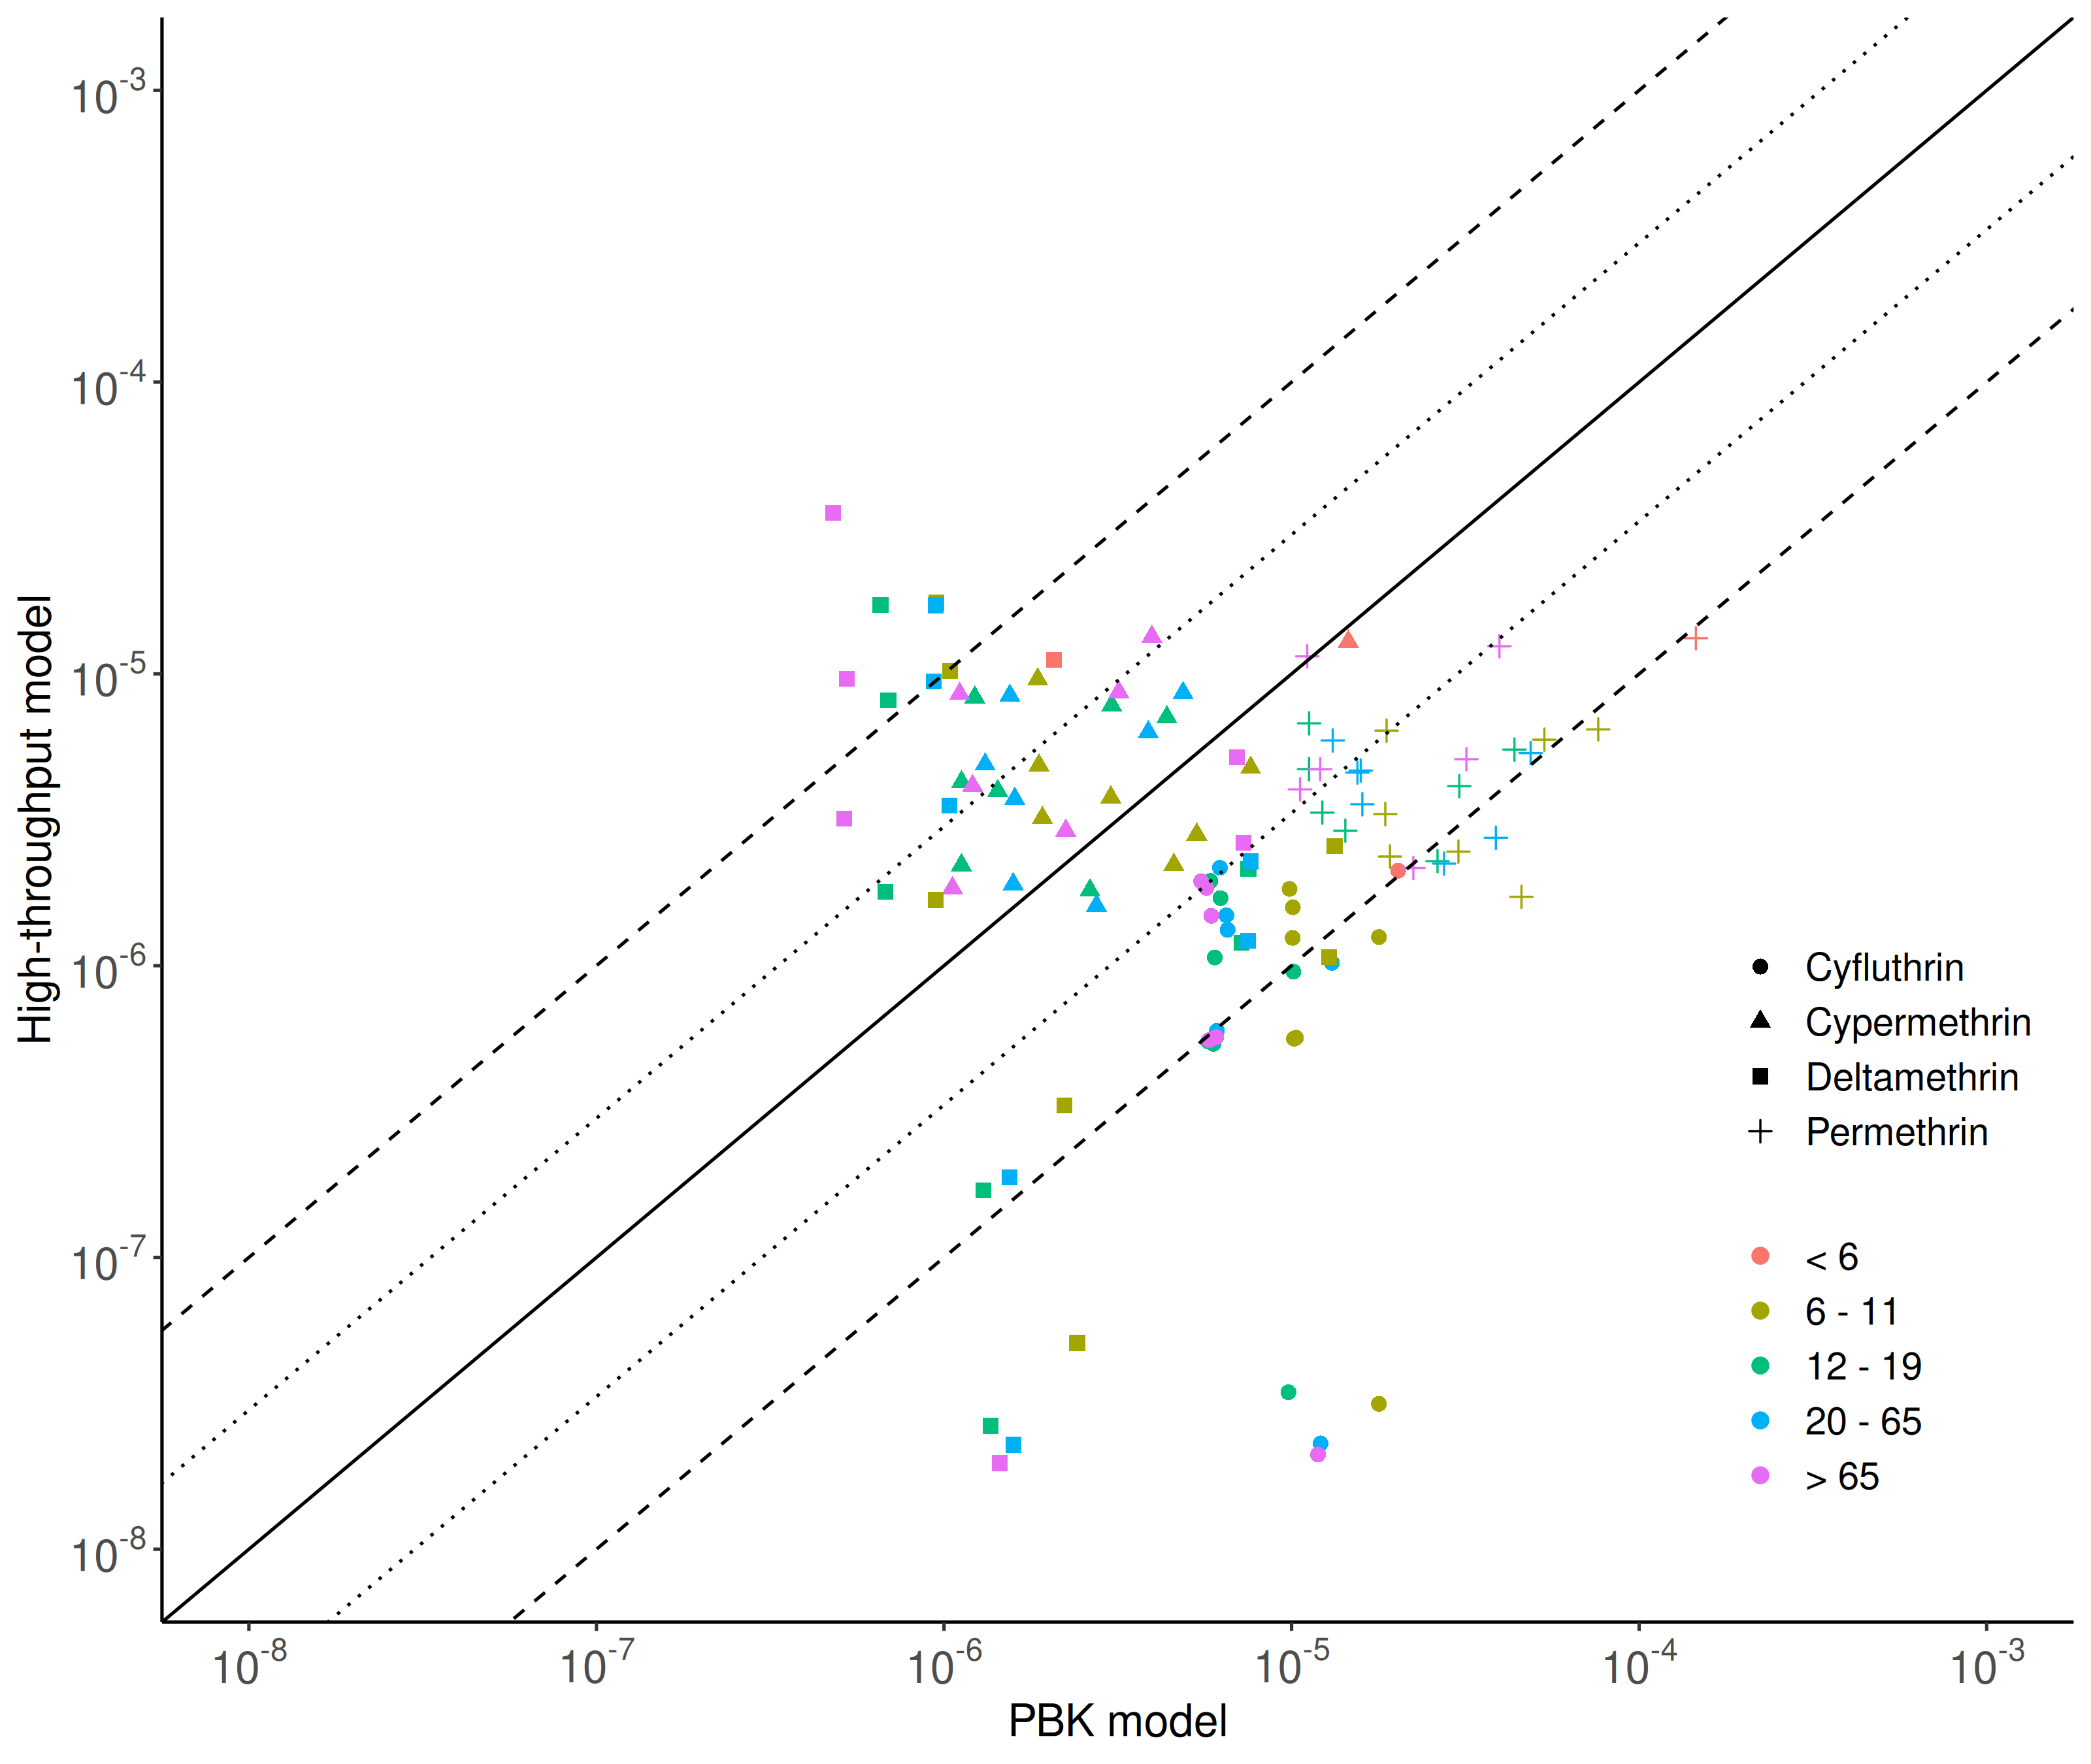
\includegraphics[width=\linewidth]{figures/fig4}
\hfill
\caption{Comparison of exposure predictions from the PBK model and
high-throughput approaches, highlighting similarities and discrepancies. The
solid line represents a perfect match between the two methods, while dotted and
dashed lines indicate errors within three- and ten-fold differences,
respectively.\label{fig:fig4}}
\end{figure}

The cross-comparison of exposure dose predictions based on different
tools is detailed in Supplementary Materials File S1. Briefly, using
average food residue data (mg/kg food) from the United States Department
of Agriculture (USDA) Pesticide Data Program (PDP) database (2002--2011)
and consumption data (g food/kg bw/day) for individuals aged 6--79 from
the U.S. EPA Food Commodity Intake Database (2005--2010),
\citet{aylward_screening_level_2018} estimated the exposures of
permethrin, cypermethrin, and deltamethrin to be
\(1.83 \times 10^{-3}\), \(6.1 \times
10^{-4}\), and \(1.9 \times 10^{-6}\) mg/kg-d, respectively. In the U.S.
EPA report, intake estimations are based on the Dietary Exposure
Evaluation Model (DEEM) Software with Food Commodity Intake Database,
which uses 2003-2008 food consumption data from the USDA's National
Health and Nutrition Examination Survey, What We Eat in America
(NHANES/WWEIA). The SEEM approach, validated by NHANES data, provides
exposure estimates similar to those based on biomonitoring data.
According to the latest U.S. EPA reports, across all age groups and
pyrethroid pesticides, the population-adjusted dose (PAD) shows that
cyfluthrin and beta-cyfluthrin presents the highest acute dietary risk
estimate for children aged 1-2, which uses 96\% of the acute PAD. The
risk estimates of PAD are reported at the 99.9th and 50th percentiles
for acute and chronic exposure. By contrast, biomonitoring data-driven
intake rates have \%PAD values of less than 2\%. Additionally, using
food consumption data, the predicted intake of pyrethroids is about an
order of magnitude higher than predictions from biomonitoring data.
Regardless of the tools employed, children typically exhibit the highest
estimated exposure levels compared to other age groups. It is important
to note that DPR's own process of assessing risk from dietary exposure
does not use 50th percentile approach for estimating chronic exposure,
but rather more refined consumption estimates based on the available
data.

\subsection{Exposure variability, trend, and
similarity}\label{exposure-variability-trend-and-similarity}

We selected 3PBA to assess variability and difference in reverse
dosimetry because it was the only compound with a detection rate over
60\%. Preliminary examination showed that the coefficient of variance
for 3PBA was over 33\%, corresponding to the expecting concerns about
data reliability \citep{faure_evaluation_2020}. Figure \ref{fig:fig5}
shows the differences in P95/P50 across age groups for 3PBA and
permethrin. The highest predicted ratio (19.8) for 3PBA was observed in
the 6-11 age group during 1999-2000. In comparison, the ratio for
permethrin in the same group was estimated to be 10.7, indicating a
twofold difference between the P95/P50 values, possibly due to other
unknown factors (e.g., inter-individual variability). Across all cohorts
and age groups, the P95/P50 for 3PBA ranged from 7.0 (6-11 years old;
2013-2014) to 19.8, reflecting wide inter-individual variation in dose
rates and the low half-life and exposure interval ratio. Overall, the
ratio for 3PBA is higher than that for its parent compound, permethrin,
which P95/P50 ranged 4.9 (6-11 years old; 2011-2012) to 17.8 (12-19
years old; 2007-2008). The factor of P95/P50 difference between 3PBA and
permethrin ranged from 0.8 (\textgreater65 years; 2007-2008) to 2.09
(12-19 years old; 2015-2016), with no significant differences across age
groups.

\begin{figure}[H]
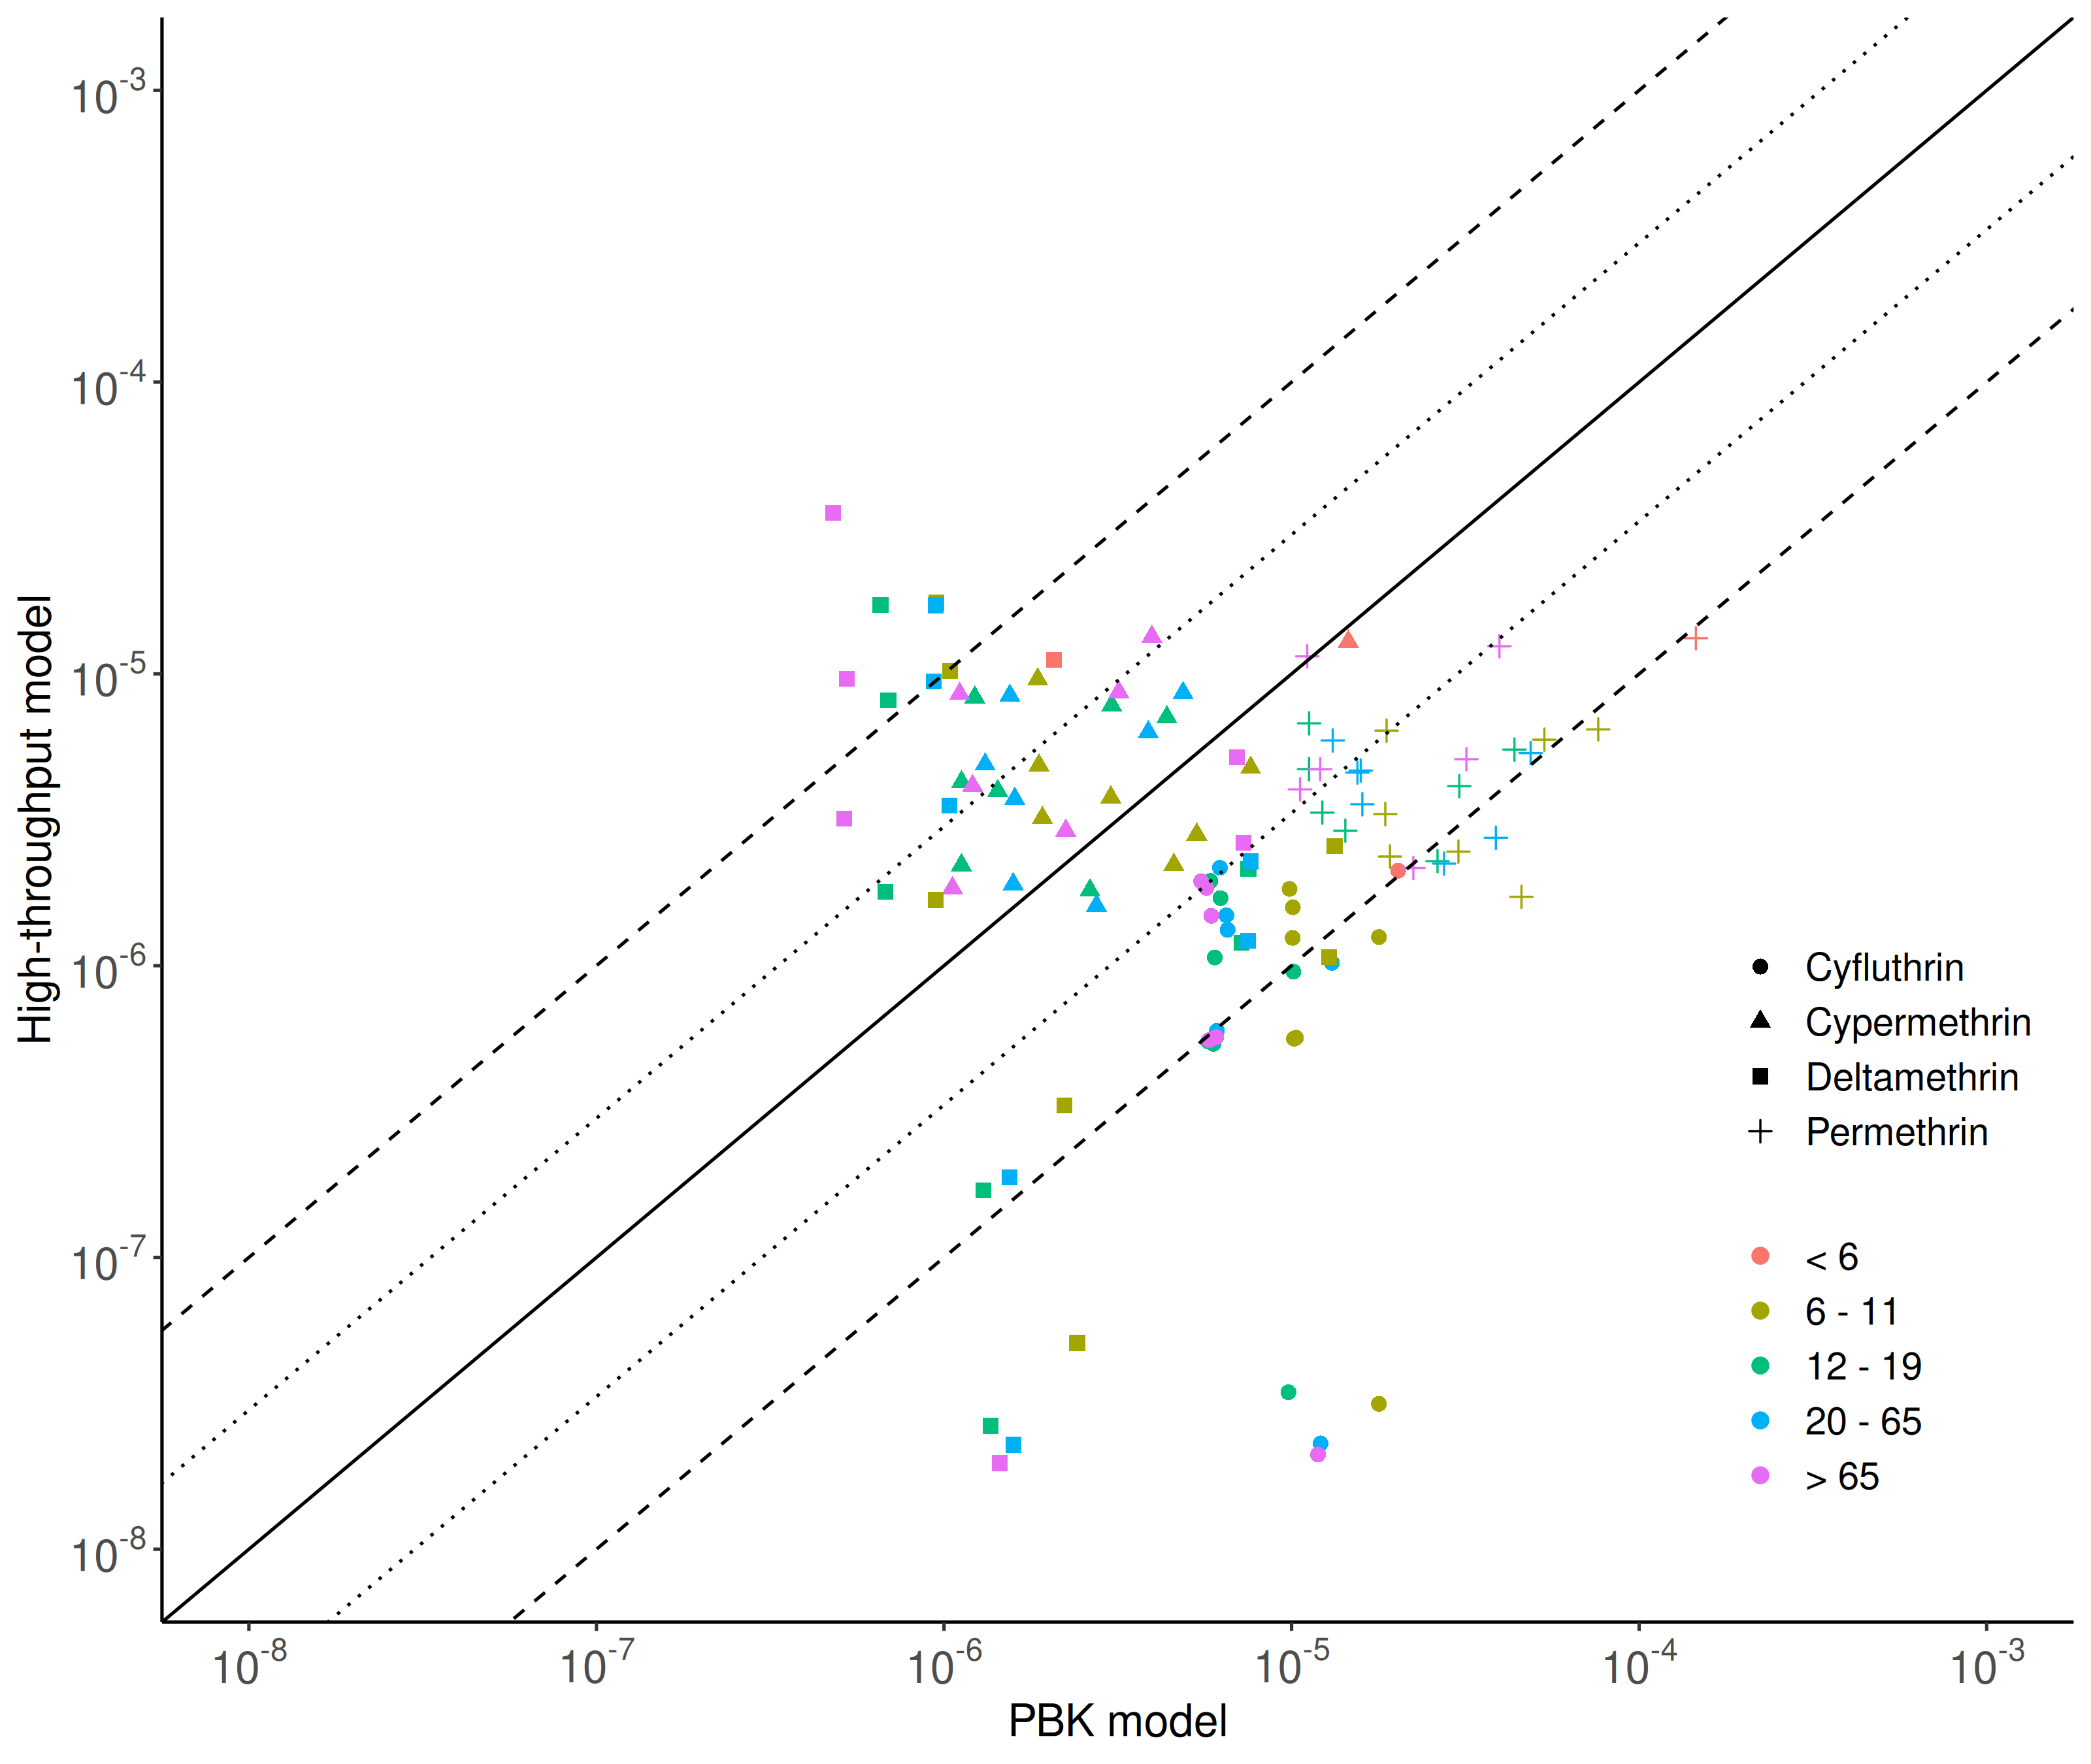
\includegraphics[width=1\linewidth,]{figures/fig5} \caption{Variability in exposure estimates across age groups. Variability in exposure is shown using P95/P50 ratios for 3PBA and permethrin across age groups. Greater variability is observed in the high differences between permethrin and 3PBA in the top panel, as well as in the larger dots depicted in the lower panel.}\label{fig:fig5}
\end{figure}

Our study also investigated the exposure trend based on the 3PBA
biomonitoring data and its related parent compound. As mentioned, the
detection rate has significantly increased in recent years. Figure
\ref{fig:fig6} shows the geometric mean of 3PBA and the predicted daily
intake rate of permethrin, estimated by the PBK and high-throughput
models across all cohorts from 1999 to 2016. Permethrin was selected due
to the highest detection rate of 3PBA and the completeness of the
investigation across all cohorts. According to the urine 3PBA data,
there was an increasing exposure trend from 1999 to 2016. Compared to
earlier surveys, the geometric mean of urine 3PBA was about two-fold
higher in the 2015-2016 investigation than in 1999-2000. In our
prediction, the PBK model showed an exposure trend with an intake rate
increment of less than an order of magnitude. However, unlike the PBK
model, the high-throughput approach could not provide an exposure trend.
Nonetheless, a common finding was that children under 6 years old had
the highest exposure compared to other population subgroups. This result
could not be obtained by exploring only the urine 3PBA data.

\begin{figure}[H]
\centering
\begin{adjustwidth}{-2cm}{}
\centering
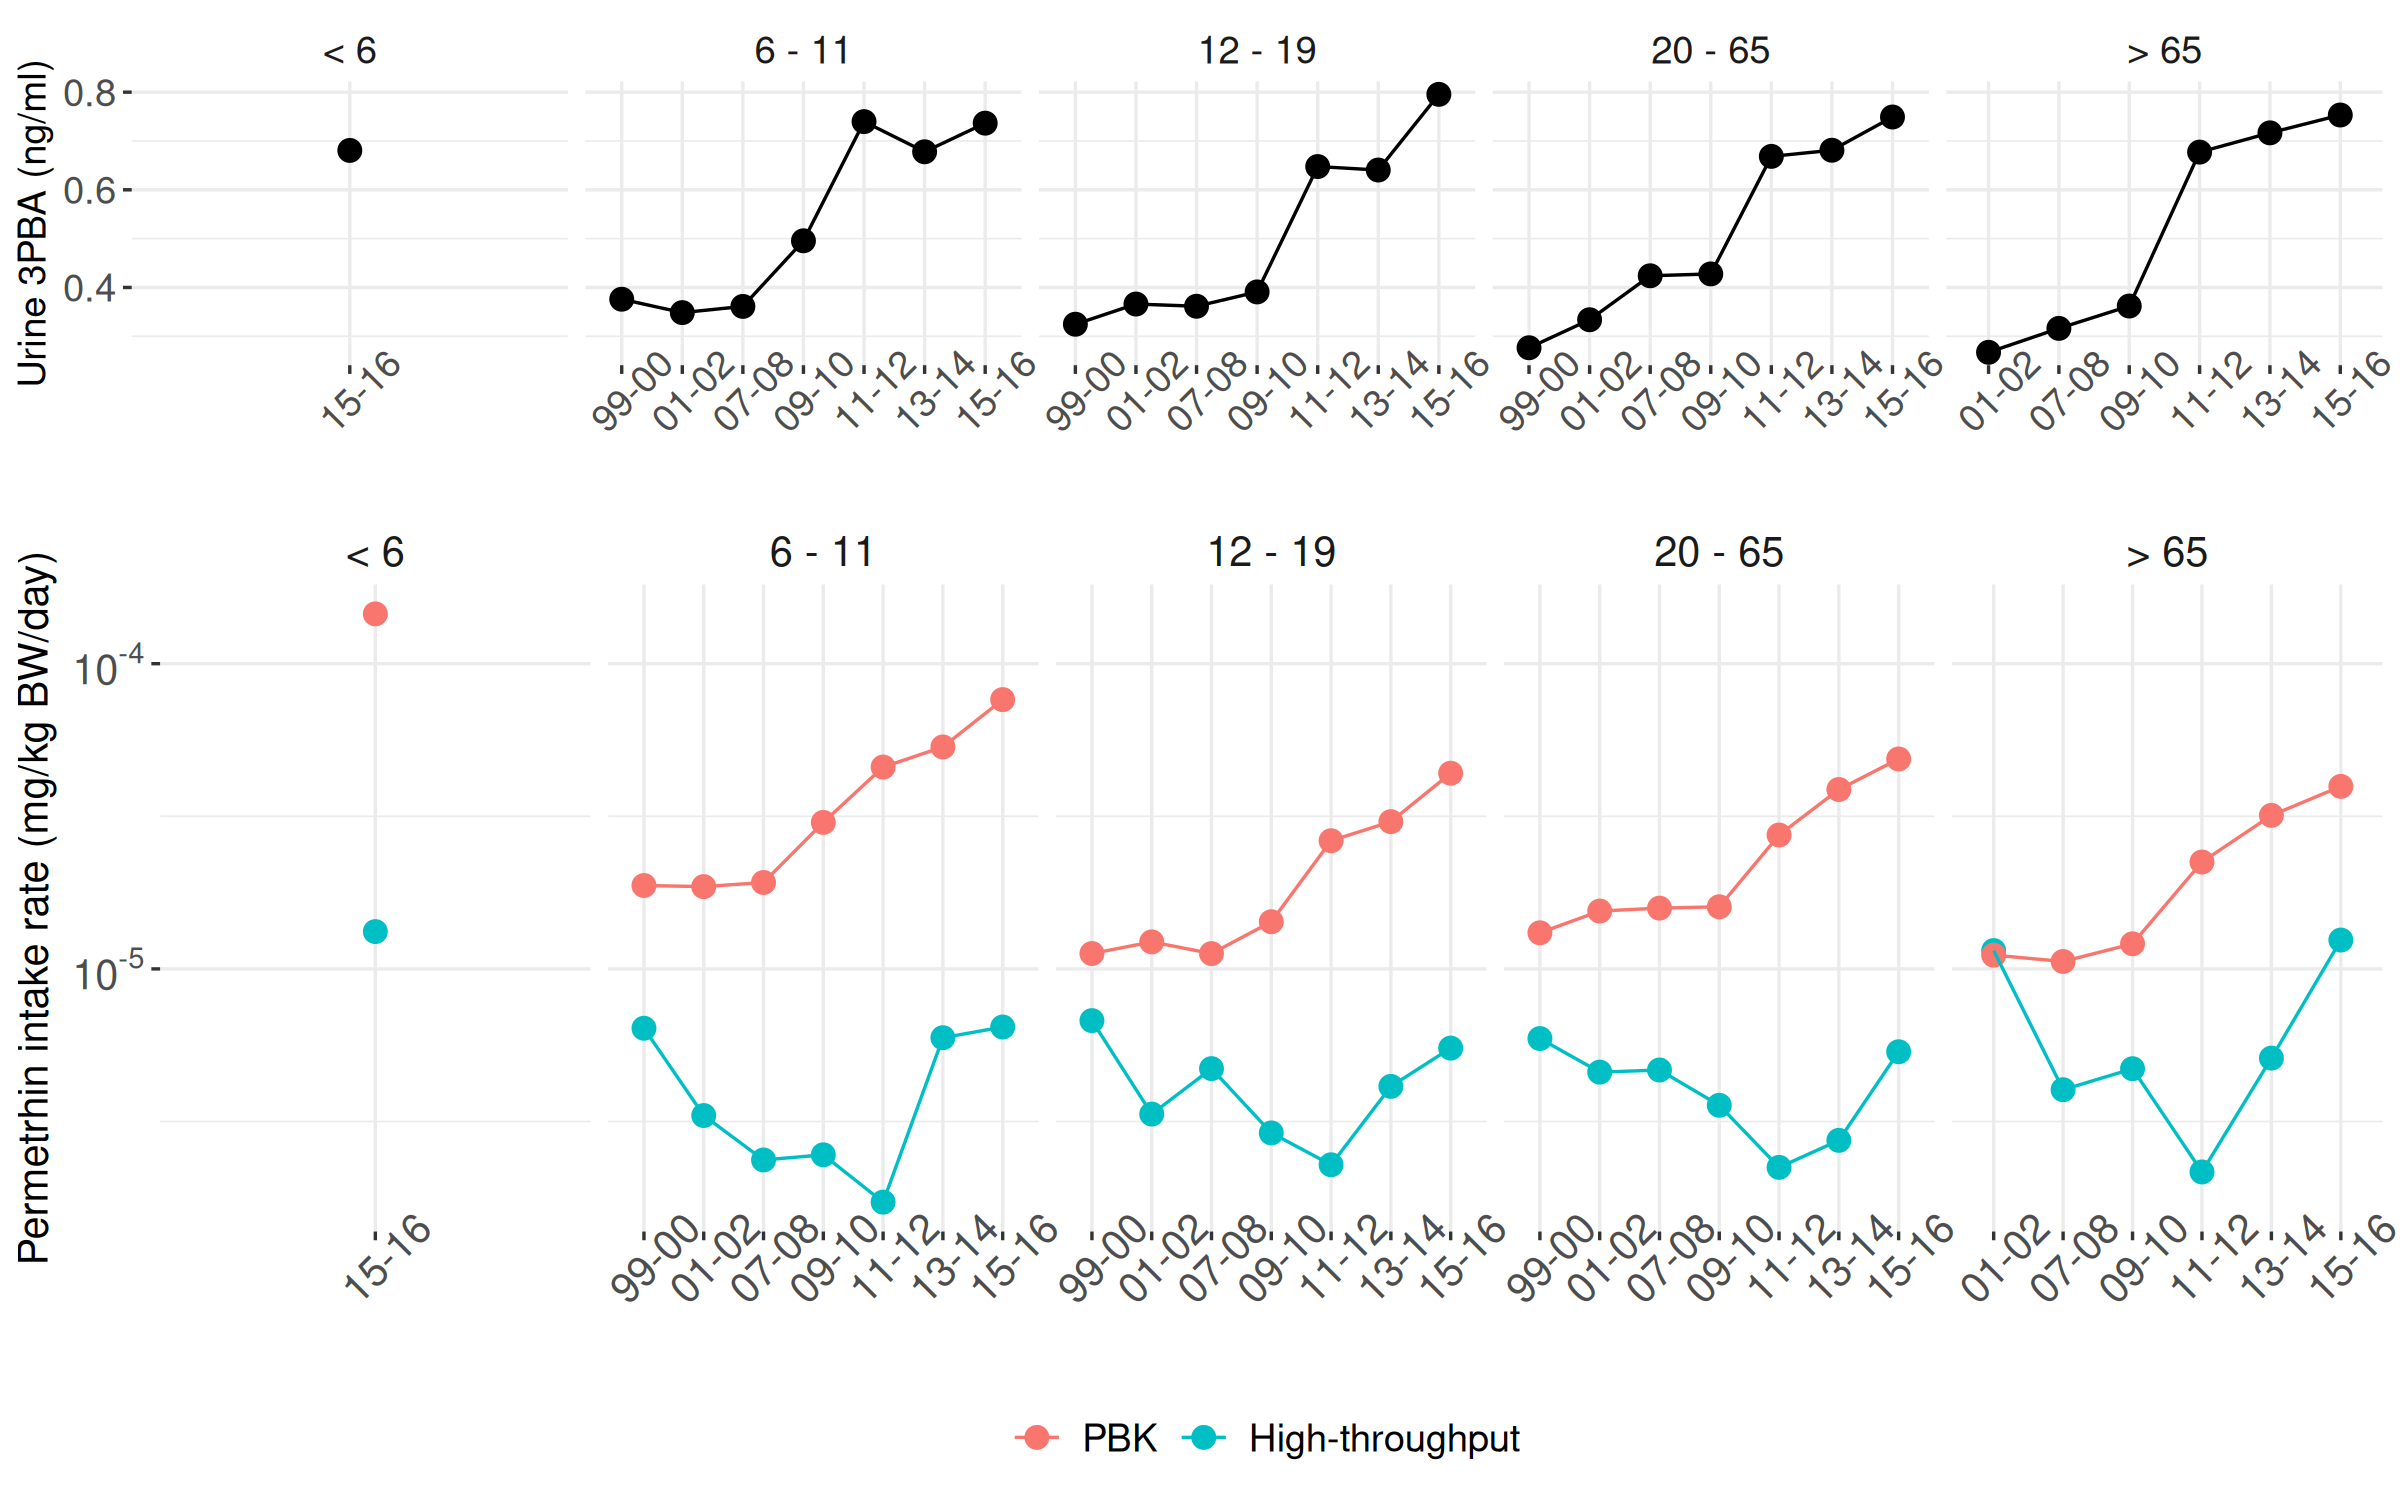
\includegraphics[width=\linewidth]{figures/fig6}
\hfill
\end{adjustwidth}
\caption{Trends in urinary 3PBA (top) and derived permethrin daily intake (bottom) from 1999
to 2016. Predicted intakes are shown separately for physiologically based
kinetic and high-throughput models.\label{fig:fig6}}
\end{figure}

To identify specific exposure patterns, the median exposure estimates
for each population group from each cycle were used to examine exposure
similarity (Figure \ref{fig:fig7}). The results show that the children
aged \textless6 and between 6-11 years exhibited similar exposure
patterns, compared to other four age groups over 12 years old. Overall,
our results indicate higher exposure levels in younger populations,
consistent with other prediction tools shown in Supplementary Materials
File S1.

\begin{figure}[H]
\centering
\begin{adjustwidth}{-2cm}{}
\centering
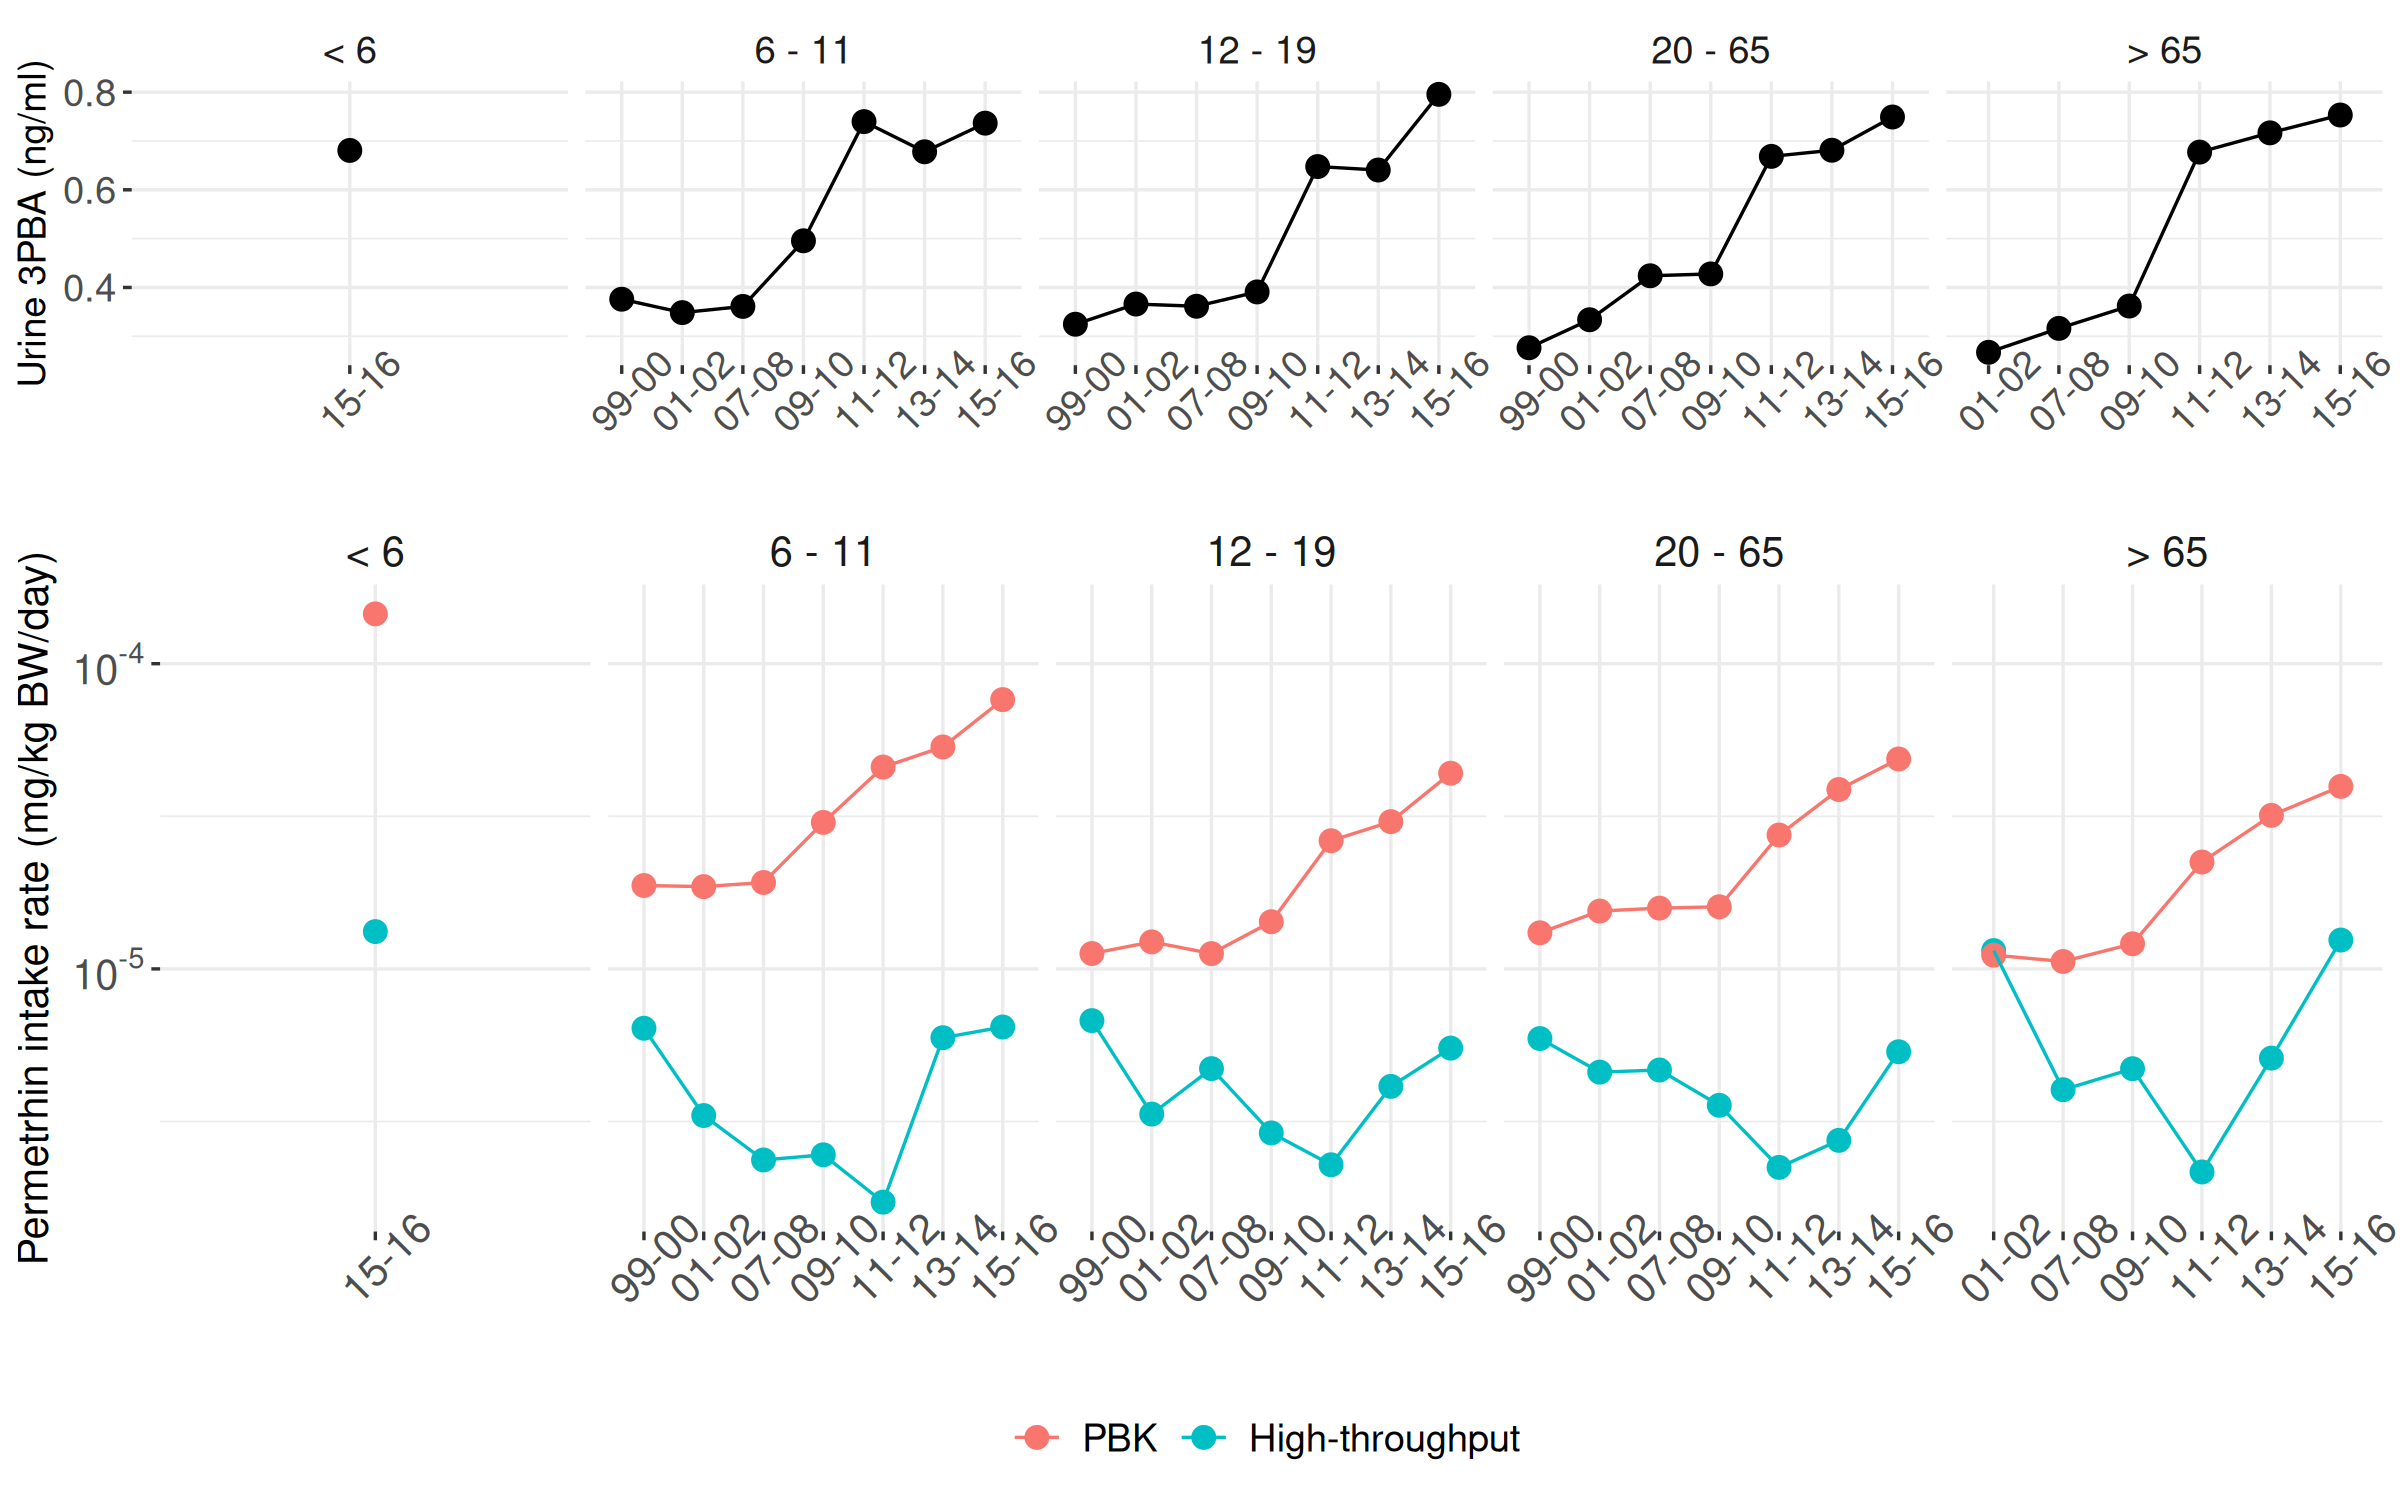
\includegraphics[width=\linewidth]{figures/fig7}
\hfill
\end{adjustwidth}
\caption{Exposure similarity across age groups. Age groups are arranged by
class, highlighting similar exposure levels across NHANES cycles.\label{fig:fig7}}
\end{figure}

\subsection{Risk assessment}\label{risk-assessment}

Exposure predictions from the PBK model revealed that the highest annual
exposure to deltamethrin occurred in the 6-11 age group during the
2009-2010 NHANES cycle. For permethrin and cyfluthrin, the highest
exposure levels were observed in children under 6 years old during the
2015-2016 cycle. To establish a conservative protective strategy,
exposure values from the top 1\% of each group were used to calculate
the Margin of Exposure (MOE) and the systematic exposure-derived Margin
of Internal Exposure (MOIE). Bayesian inference estimates showed that
the geometric mean population oral intake rates for deltamethrin,
permethrin, and cyfluthrin were \(3.83 \times 10^{-5}\) mg/kg-day (GSD =
1.09), \(2.25 \times 10^{-3}\) mg/kg-day (GSD = 1.13), and \(6.79 \times
10^{-5}\) mg/kg-day (GSD = 1.11), respectively. The intake rate for
cypermethrin was estimated at \(2.25 \times 10^{-4}\) mg/kg-day based on
the intake rate of permethrin.

Using the Bayesian BMD model, the estimated Benchmark Dose Lower
Confidence Limits (BMDL) were determined as 1.79 mg/kg for deltamethrin,
39.17 mg/kg for permethrin, 5.48 mg/kg for cypermethrin, and 1.22 mg/kg
for cyfluthrin. Rat PBK modeling provided Cmax and AUC values in plasma
and brain tissue for each compound. For deltamethrin, the plasma Cmax
and AUC were 118.2 ng/mL and 1174.1 ng-h/mL, respectively, while the
brain values were 34 ng/g and 475 ng-h/g.

Following Wolansky's findings of a 40\% cis and 60\% trans isomer
composition for permethrin, the plasma Cmax and AUC for cis-permethrin
were 1605.5 ng/mL and 15,822.6 ng-h/mL, with brain values of 459.8 ng/g
and 6400 ng-h/g. For trans-permethrin, the plasma Cmax and AUC were 503
ng/mL and 4926.1 ng-h/mL, while brain values were 143.8 ng/g and 1996.4
ng-h/g.

In the absence of specific TK data and PBK parameters
for cyfluthrin and cypermethrin, chemical-specific parameters from
deltamethrin were used to estimate dose metrics. For cis-cyfluthrin, the
plasma Cmax and AUC were 32.18 ng/mL and 319.8 ng-h/mL, while brain
values were 9.26 ng/g and 129.4 ng-h/g. For trans-cyfluthrin, the plasma
Cmax and AUC were 48.3 ng/mL and 479.8 ng-h/mL, with brain values of
13.9 ng/g and 194.1 ng-h/g.

For cis-cypermethrin, the plasma Cmax and AUC were 152.2 ng/mL and
1510.8 ng-h/mL, while brain values were 43.7 ng/g and 611.2 ng-h/g. For
trans-cypermethrin, the plasma Cmax and AUC were 210.4 ng/mL and 2087.9
ng-h/mL, with brain values of 60.5 ng/g and 845.7 ng-h/g.

Figure \ref{fig:fig8} illustrates the estimated probability
distributions of the MOE and MOIE for pyrethroid pesticides, based on
external exposure and the associated dose metrics. Overall, all
estimated values exceeded \(1.0 \times 10^{4}\), indicating an
acceptable level of acute risk under exposure conditions derived from
biomonitoring data. Notably, MOEs calculated from oral doses were lower
than MOIEs derived from internal doses, highlighting that conventional
external exposure assessments tend to overestimate risk compared to
advanced internal dose-based techniques.

\begin{figure}[H]
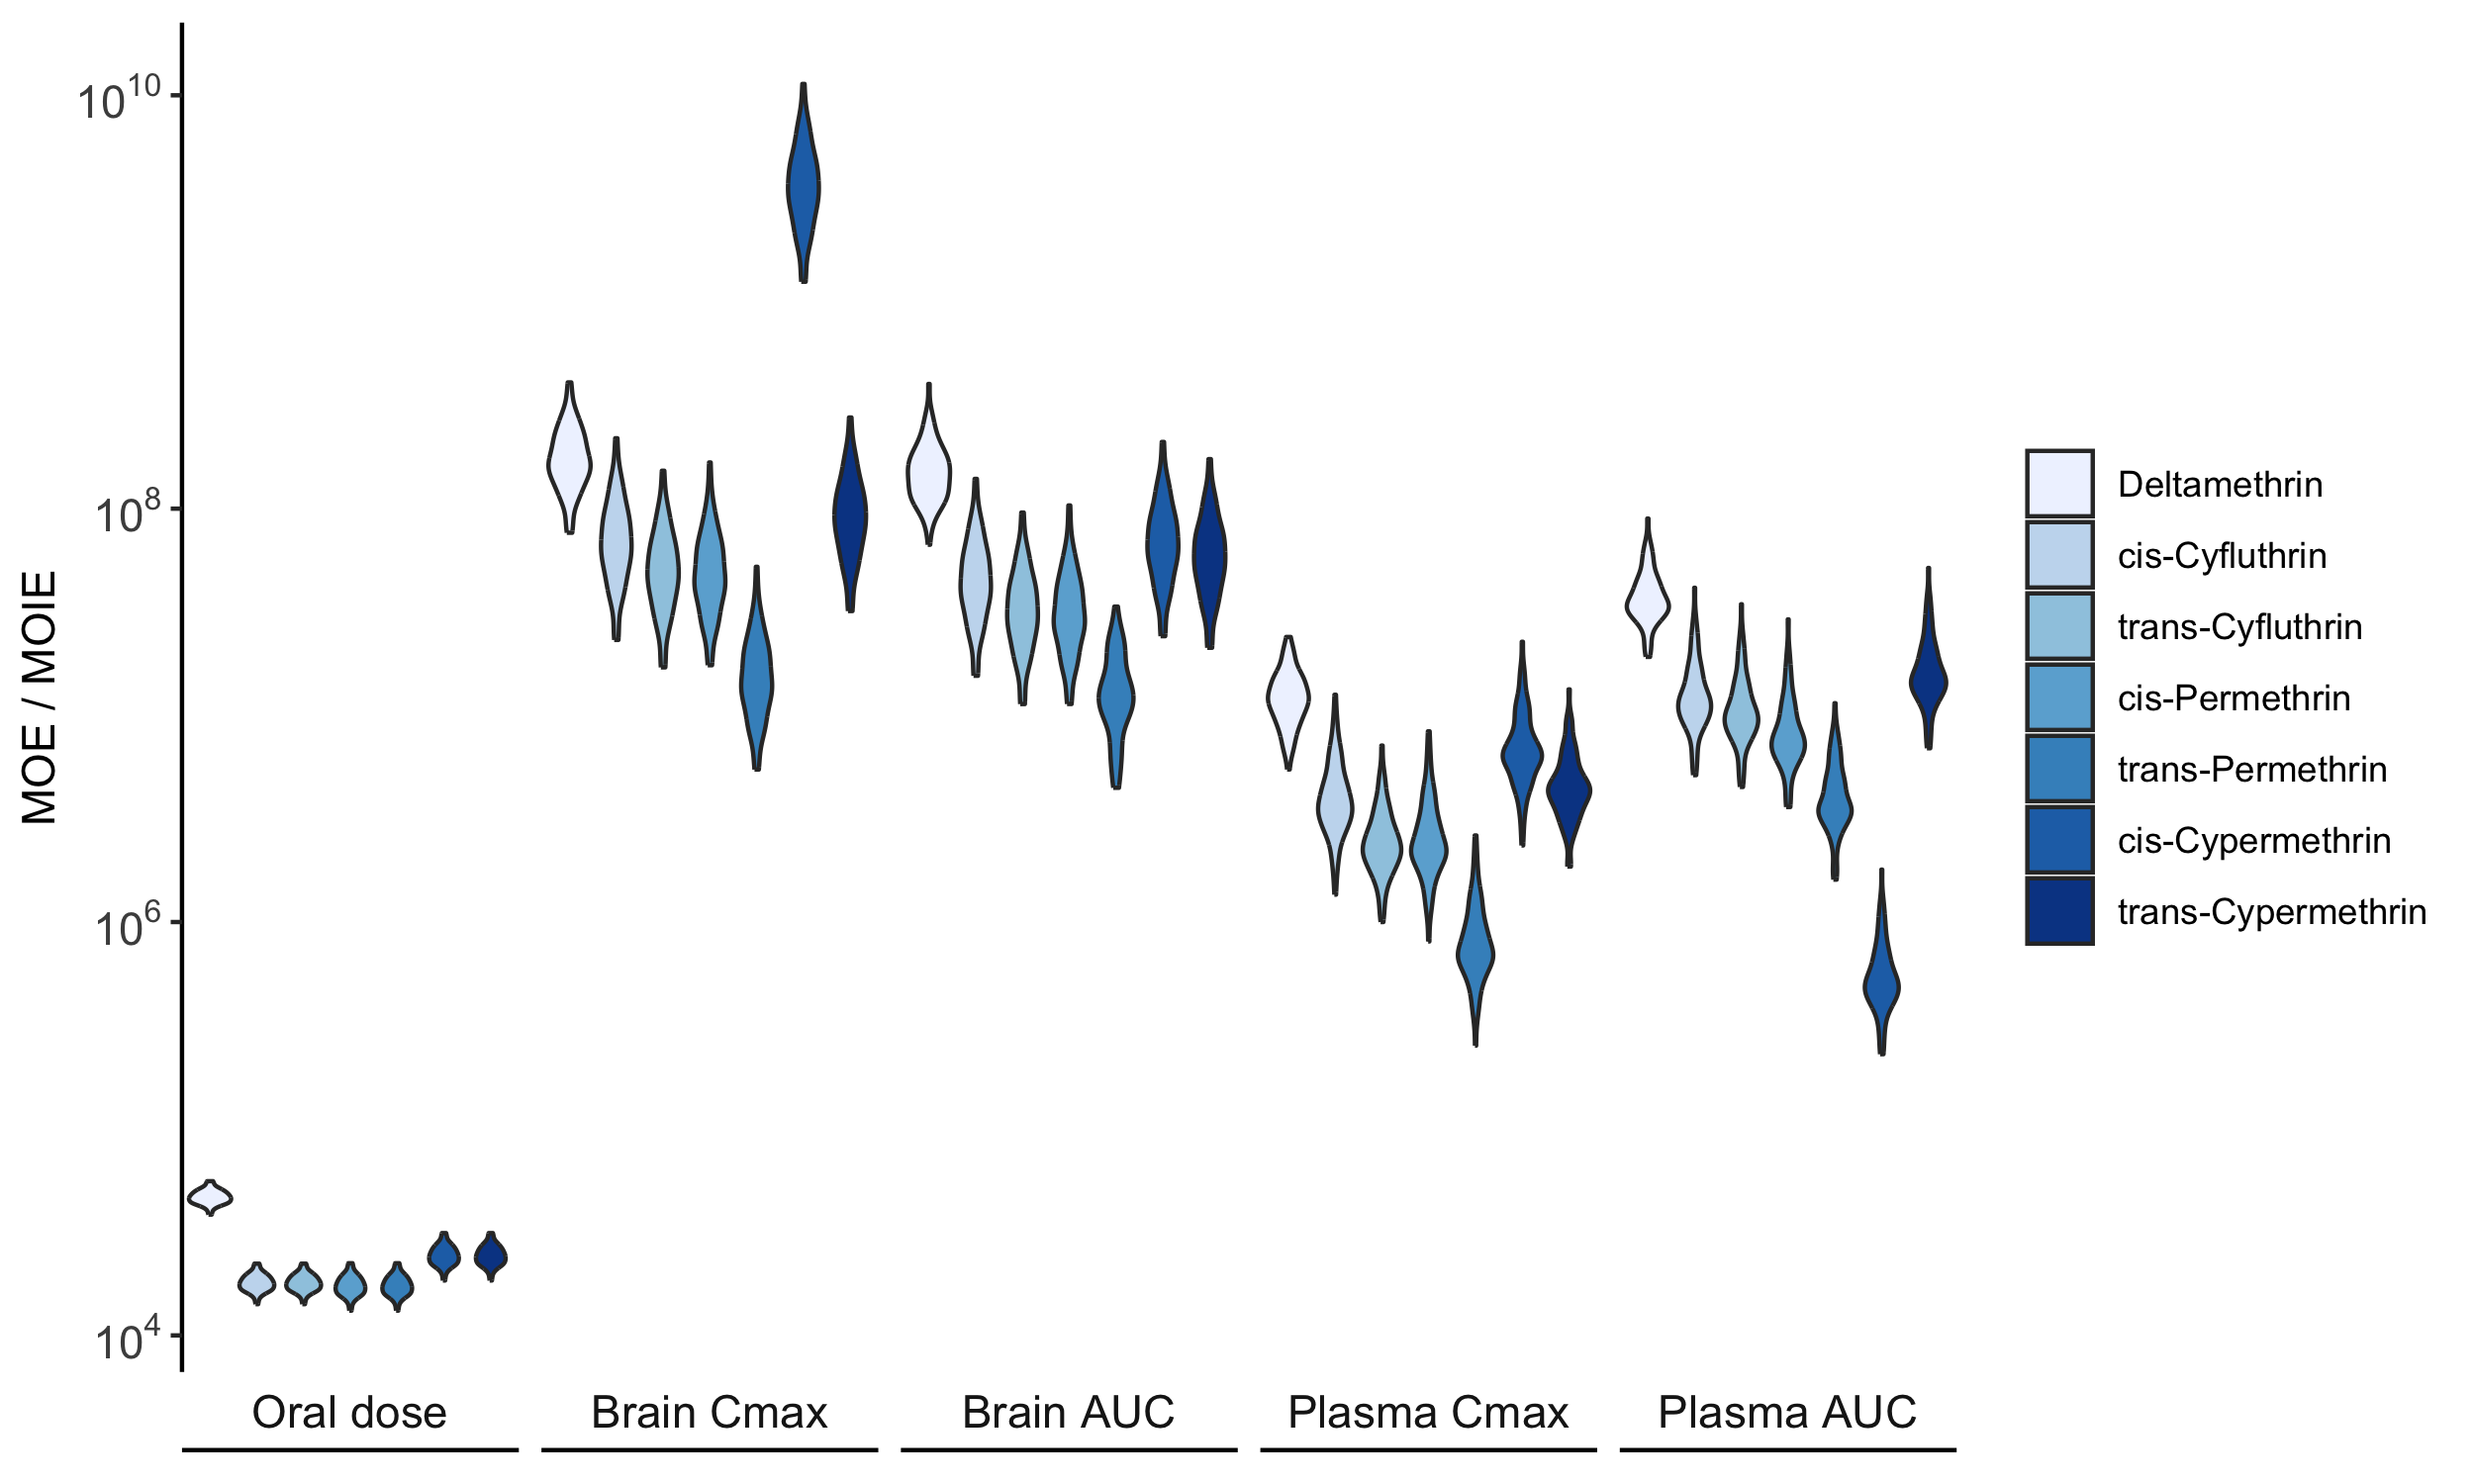
\includegraphics[width=1\linewidth,]{figures/fig8} \caption{Distribution of the margin of exposure (MOE) and margin of internal exposure (MOIE) for acute neurotoxic effects calculated from daily oral and corresponding systematic exposure, respectively. Higher MOE or MOIE values indicate a lower exposure risk.}\label{fig:fig8}
\end{figure}

%%%%%%%%%%%%%%%%%%%%%%%%%%%%%%%%%%%%%%%%%%
\section{Discussion}

In this study, we successfully refined a PBK model to reconstruct
exposure patterns from publicly available biomonitoring data of
pyrethroid metabolites within the U.S. population. This methodology
aligns with the previous approaches used for methylmercury and
chloroform, where the focus was on a single model without comparative
exposure assessments, potentially compromising reliability
\citep{allen2007use, lyons2008computational}. Our study rectifies this
by benchmarking PBK model predictions against other exposure prediction
tools, thus reinforcing the PBK model's robustness and applicability in
exposure assessment.

It is noteworthy that we reused of human TK data from earlier model
development, which is critical for robust predictions in our model
verification. While we did not introduce major structural changes to the
existing model, we validated its performance with the same TK data to
ensure model reliability. Our refined PBK model demonstrated similar
predictability to the global pyrethroid model by
\citet{quindroit2021estimating}, with approximately 65\% and 75\% of
predictions falling within 2-fold and 3-fold error intervals,
respectively. The model developed by \citet{quindroit2021estimating}
only applied to simulate the pyrethroids concentration for adult group,
our refined model aims to apply the exposure prediction to different age
groups, including children.

This study primarily compares daily intake estimates with the
high-throughput modeling approach, utilizing NHANES biomonitoring data
for exposure estimation. Bayesian inference was applied to quantify
uncertainty in both methods. Previous studies that excluded outliers to
avoid acute exposure under atypical conditions
\citep{bao2020association}, our study included all observations,
providing a comprehensive depiction of exposure. The Bayesian
probabilistic approach's flexibility was instrumental in achieving this
goal. The Bayesian method also has the capability to include the data
that is under LOD in providing proper inference.

Generally, PBK model tends to estimate higher exposure levels than the
high-throughput approach due to the inclusion of chemical-specific
bioavailability parameters. Lower detection rates for key metabolites
such as DBCA and FPBA led to inconsistencies in predictions for
deltamethrin and cyfluthrin compared to permethrin and cypermethrin,
with less than 60\% of predictions within a 10-fold difference. The lack
of DBCA data in the recent cycles (after 2009-2010) further complicated
these predictions. Despite these challenges, both methods consistently
indicated higher pyrethroid exposure levels in children compared to
other age groups, corroborating findings from other studies using
dietary intake from food commodity in exposure prediction. Newly
available NHANES data (2015-2016) for children aged 3-5 have the highest
exposure compared to the older age groups.

Advanced research by \citet{stanfield2024characterizing} supports the
high-throughput approach's capability to detect exposure trends. In
addition, using food consumption data, the predicted intake of
pyrethroids is approximately ten times higher than the predictions
derived from biomonitoring data. This discrepancy suggests that
biomonitoring assessments, which rely on detecting major urine
metabolites, may underestimate exposure. This underestimation occurs if
these metabolites, assumed to be stable first-generation products,
without undergoing further metabolism. For instance, exposure to
cyfluthrin might be underestimated if its metabolite, DCCA, continues to
be metabolized further.

Our exposure prediction closely aligned with the findings of the France study
\citep{quindroit2021estimating}, which also employed a physiologically based
kinetic (PBK) approach. The Fance study estimated median daily intakes of 
\(3.4 \times 10^{-5}\), \(8.1 \times 10^{-4}\), \(2.0 \times 10^{-5}\), and
\(1.8 \times 10^{-5}\) mg/kg-day for deltamethrin, permethrin, cyfluthrin, and
cypermethrin, respectively. Additionally, no risks were anticipated from the
reconstructed pyrethroid exposures. Furthmore, a China study found that
metabolite levels among 481 infants were similar or slightly higher than in the
U.S. population \citep{wu2013urinary}.

Previous research shows that chronic NOAELs are similar to or higher
than the acute POD used in this study
(\url{https://www.regulations.gov/document/EPA-HQ-OPP-2009-0637-0036}).
For deltamethrin, the chronic dog oral intake study (1 mg/kg/day) and
Wolansky et al. \citep{wolansky_relative_2006} (0.99 mg/kg) have very
similar PODs, which are among the lowest available. Therefore, POD of
approximately 1 mg/kg should be protective of both acute and long-term
effects. It is crucial to note that the BMDLs used in the current study
are higher than the lower confidence limit of threshold dose estimated
in \citep{wolansky_relative_2006}, whose benchmark response was a 30\%
reduction in motor activity versus one standard deviation of the control
value selected by the U.S.EPA. However, the Bayesian statistical
approach had been proof to have higher capability in determine the
regulation than the traditional frequentist method to estimate the
robust BMD in risk analysis and further regulation
\citep{desai_role_2024}.

This study specifically focused on acute exposure risks. Due to the short
half-life of pyrethroids, predicting exposure based on a steady-state
assumption introduces significant uncertainty. Previous research has indicated
that children's exposures are more likely to be episodic rather than fostering
a steady-state condition \citep{kissel_comparison_2005}. As noted earlier, risk
estimates derived from acute exposure and associated endpoints are generally
sufficient to address risks from repeated or long-term exposures, though they
are less suitable for reconstructing chronic exposure patterns
\citep{hays2007biomonitoring, aylward_interpreting_2012}. Furthermore, the U.S.
EPA's risk assessment identified no cumulative risks of concern for pyrethroid
pesticides
(\url{https://www.regulations.gov/document/EPA-HQ-OPP-2011-0746-0003}). Due to
the lack of increased toxicity from repeated/chronic exposure to pyrethroid,
the risk estimates derived from use of the acute study are adopted to protect
the risk from repeated exposures. In addition, the current experiment data for
acute toxicity was the most robust data set for assessing exposure and risk.

In a risk assessment based on data from the Canadian Health Measures
Survey and using neurotoxic effects as the endpoint,
\citet{faure_evaluation_2020} reported that the hazard quotient of 3PBA
exceeded 1. However, while 3PBA is a metabolite of several pyrethroids
with varying toxicities, the metabolite itself is considered less toxic.
As a result, reverse dosimetry is required to investigate the parent
compounds present in target tissues. Our research showed that in a
similar geographical context, all estimated MOEs for the U.S. population
exceeded \(1.0 \times 10^{4}\), contrasting with the findings of the
Canadian study and indicating that pyrethroid exposure among the general
U.S. population is at an acceptable level.

Unlike most studies that conduct health risk assessments using urinary
concentrations or intake dose rates, our study utilized a
physiologically based kinetic (PBK) model to assess risk based on dose
metrics in the brain and plasma, which are directly associated with
neurotoxic health effects. Our study approach is similar to a study by
\citet{arnot_developing_2022}, who applied the internal threshold of
toxicological concern to compare the no observed effect level (NOEL)
from oral intake and whole-body exposure.

There are certain limitations in the PBK dose reconstruction. In the
refined PBK model, the parameters were based on earlier studies without
further modification. Consequently, because the original model was
constructed primarily based on animal and human studies of deltamethrin
and permethrin, parameters for cyfluthrin and cypermethrin were sourced
from in vitro and in silico studies or extrapolated from the other two
pyrethroids \citep{quindroit2019estimating}, resulting in observational
and predictive differences over a factor of 3. Exposure predictions from
biomarkers are generally lower than those from dietary sources. Due to
the relatively short half-lives of pyrethroids, it is likely to
underestimate intake rates through spot urine samples from NHANES.
Additionally, \citet{barr2010urinary} indicated that morning samples had
significantly higher concentrations than those collected in the
afternoon and evening. 

Sampling time, frequency, and detection limits significantly influence the
accuracy and interpretation of biomonitoring data, affecting predictions of
chemical intake \citep{hays2007biomonitoring}. Specifically, 1) the timing of
sample collection impacts measured concentrations of chemicals and their
metabolites. For pyrethroids, which have short biological half-lives, urinary
levels fluctuate markedly depending on exposure timing. Sampling too early or
too late may misrepresent actual exposure. 2) The frequency of sampling
determines how well exposure trends are captured. Spot urine samples reflect
only recent exposures and may not represent chronic levels, whereas 24-hour
collections average fluctuations for a more reliable picture.
\citet{hays2007biomonitoring} noted that peak urinary concentrations can exceed
steady-state levels by twofold, making single-spot samples less suitable for
comparison to reference values. 3) Analytical sensitivity governs the detection
of low-level exposures. High detection limits may miss subtle but significant
exposures, underestimating risk, while overly sensitive limits might detect
trace, biologically irrelevant levels, potentially raising undue concern.
Together, these factors shape the reliability of biomonitoring results and
their use in exposure prediction.

The PBK model provides an opportunity to estimate chemical-specific human
variability TK adjustment factors to replace the default uncertainty factor of
3.16 \citep{chiu_advancing_2018}. However, this method did not work in the
present study since the only uncertainty/variability is from exposure. In the
modeling process, unlike high-throughput model, the PBK model needs adequate
animal experiment data to develop the robust model in exposure prediction.

Regarding to the data availability, the newly accessible biomonitoring
data from NHANES used in the current study lags by nearly a decade. This
delay in data availability limits its ability to reflect recent exposure
trends in a timely manner. Consequently, alternative data sources, such
as pesticide use reports (e.g., PUR data from the California DPR) and
regional investigations, can serve as valuable tools for understanding
and predicting exposure trends.

This study refined the pyrethroid PBK model and identified potential
future applications. For example, it is preferable to use a PBK model to
derive relative potency factors based on internal dosimetry.
\citet{quindroit2021estimating} and \citet{thepaut_pbpk_2024} applied
the PBK model in cumulative risk assessment, though their study was
based on intake dose rate rather than internal dose in target organs
related to toxicity endpoints. The updated model was used to estimate
and update the Tier 1 provisional biomonitoring equivalent in
\citet{aylward_screening_level_2018} for assessing population urinary
3PBA data. The Tier 1 value was used for evaluating population
biomonitoring data for 3PBA in the context of a conservative cumulative
risk assessment for a group of pyrethroid compounds.

In conclusion, the refined PBK model substantially enhances the
understanding of pyrethroid-associated health risks, providing reliable
estimates and identifying critical exposure trends. This study
underscores the model's potential for broader applications in health
risk assessments and highlights the need for ongoing research and
regulatory updates to safeguard public health. By continuously improving
exposure models and integrating comprehensive biomonitoring data, we can
better protect vulnerable populations from potential health risks
associated with pyrethroid insecticides.


%%%%%%%%%%%%%%%%%%%%%%%%%%%%%%%%%%%%%%%%%%
\vspace{6pt} 

%%%%%%%%%%%%%%%%%%%%%%%%%%%%%%%%%%%%%%%%%%
%% optional
\supplementary{The following supporting information can be downloaded at:  \linksupplementary{s1}, Table S1: Summary of exposure predictions from this study and other predicted approaches.}

% Only for journal Methods and Protocols:
% If you wish to submit a video article, please do so with any other supplementary material.
% \supplementary{The following supporting information can be downloaded at: \linksupplementary{s1}, Figure S1: title; Table S1: title; Video S1: title. A supporting video article is available at doi: link.}

% Only used for preprtints:
% \supplementary{The following supporting information can be downloaded at the website of this paper posted on \href{https://www.preprints.org/}{Preprints.org}.}

% Only for journal Hardware:
% If you wish to submit a video article, please do so with any other supplementary material.
% \supplementary{The following supporting information can be downloaded at: \linksupplementary{s1}, Figure S1: title; Table S1: title; Video S1: title.\vspace{6pt}\\
%\begin{tabularx}{\textwidth}{lll}
%\toprule
%\textbf{Name} & \textbf{Type} & \textbf{Description} \\
%\midrule
%S1 & Python script (.py) & Script of python source code used in XX \\
%S2 & Text (.txt) & Script of modelling code used to make Figure X \\
%S3 & Text (.txt) & Raw data from experiment X \\
%S4 & Video (.mp4) & Video demonstrating the hardware in use \\
%... & ... & ... \\
%\bottomrule
%\end{tabularx}
%}

%%%%%%%%%%%%%%%%%%%%%%%%%%%%%%%%%%%%%%%%%%
\authorcontributions{Conceptualization, N.H.H.; methodology, N.H.H.; software, N.H.H.; validation, N.H.H.; formal analysis, N.H.H.; investigation, N.H.H.; resources, N.H.H.; data curation, N.H.H.; writing---original draft preparation, N.H.H.; writing---review and editing, N.H.H.; visualization, N.H.H.; supervision, E.S.K.; project administration, E.S.K. All authors have read and agreed to the published version of the manuscript.}

\funding{This research received no funding from any sourcres.}

\institutionalreview{Not applicable.}

\informedconsent{Not applicable.}

\dataavailability{All biomonitoring data from NHANES can be found in the
Centers for Disease Control and Prevention's website
(\url{https://www.cdc.gov/nchs/nhanes}). The prediction from
high-throughput reverse dosimetry model can be found in the U.S.EPA GitHub repository
(\url{https://github.com/USEPA/CompTox-HumanExposure-bayesmarker}).}

% Only for journal Drones
%\durcstatement{Current research is limited to the [please insert a specific academic field, e.g., XXX], which is beneficial [share benefits and/or primary use] and does not pose a threat to public health or national security. Authors acknowledge the dual-use potential of the research involving xxx and confirm that all necessary precautions have been taken to prevent potential misuse. As an ethical responsibility, authors strictly adhere to relevant national and international laws about DURC. Authors advocate for responsible deployment, ethical considerations, regulatory compliance, and transparent reporting to mitigate misuse risks and foster beneficial outcomes.}

% Only for journal Nursing Reports
%\publicinvolvement{Please describe how the public (patients, consumers, carers) were involved in the research. Consider reporting against the GRIPP2 (Guidance for Reporting Involvement of Patients and the Public) checklist. If the public were not involved in any aspect of the research add: ``No public involvement in any aspect of this research''.}
%
%% Only for journal Nursing Reports
%\guidelinesstandards{Please add a statement indicating which reporting guideline was used when drafting the report. For example, ``This manuscript was drafted against the XXX (the full name of reporting guidelines and citation) for XXX (type of research) research''. A complete list of reporting guidelines can be accessed via the equator network: \url{https://www.equator-network.org/}.}
%
%% Only for journal Nursing Reports
%\useofartificialintelligence{Please describe in detail any and all uses of artificial intelligence (AI) or AI-assisted tools used in the preparation of the manuscript. This may include, but is not limited to, language translation, language editing and grammar, or generating text. Alternatively, please state that “AI or AI-assisted tools were not used in drafting any aspect of this manuscript”.}

\acknowledgments{This work was supported by the California Department of
Pesticide Regulation. The authors want to thank Dr.~Shelley DuTeaux and
Dr.~Gayatri Sankaran, for providing helpful comments.}

\conflictsofinterest{The authors declare no competing interests. The
views expressed in this article are those of the authors and do not
necessarily reflect the views or policies of the California Department
of Pesticide Regulation.}

%%%%%%%%%%%%%%%%%%%%%%%%%%%%%%%%%%%%%%%%%%
%% Optional

%% Only for journal Encyclopedia
%\entrylink{The Link to this entry published on the encyclopedia platform.}

\abbreviations{Abbreviations}{
The following abbreviations are used in this manuscript:\\

\noindent 
\begin{tabular}{@{}ll}
3PBA & 3-Phenoxybenzoic Acid \\
BMD & Benchmark Dose \\
BMDL & Benchmark Dose Lower Confidence Limit \\
DBCA & 3-(2,2-Dibromovinyl)-2,2-Dimethylcyclopropane Carboxylic Acid \\
DCCA & 3-(2,2-Dichlorovinyl)-2,2-Dimethylcyclopropane-1-Carboxylic
Acid \\
DPR & Department of Pesticide Regulation \\
EPA & Environmental Protection Agency \\
FPBA & 4-Fluoro-3-Phenoxybenzoic Acid \\
LOD & Limit of Detection \\
MOE & Margin of Exposure \\
MOIE & Margin of Internal Exposure \\
NHANES & National Health and Nutrition Examination Survey \\
NOEL & No-Observed-Effect Level \\
NOAEL & No-Observed-Adverse-Effect Level \\
PAD & Population-Adjusted Dose \\
PBK & Physiologically Based Kinetic \\
POD & Point of Departure \\
RfD & Reference Dose \\
SHEDS & Stochastic Human Exposure and Dose Simulation \\
TD & Toxicodynamics \\
TK & Toxicokinetics \\
USDA & United States Department of Agriculture
\end{tabular}
}

%%%%%%%%%%%%%%%%%%%%%%%%%%%%%%%%%%%%%%%%%%
%% Optional
\appendixtitles{no} % Leave argument "no" if all appendix headings stay EMPTY (then no dot is printed after "Appendix A"). If the appendix sections contain a heading then change the argument to "yes".
\appendixstart
\appendix
\section{}
\subsection{Tables}

\begin{table}[H]
\begin{adjustwidth}{-4cm}{}
  \caption{Measured pyrethroids metabolites and the limits of detection ($\mu$g/L) across each NHANES cycle.}
\label{tab:taba1}
\begin{tabular}{lrrrrrrr}
\toprule
  & 1999-2000 & 2001-2002 & 2007-2008 & 2009-2010 & 2011-2012 & 2013-2014 & 2015-2016\\
\midrule
3PBA & 0.1 & 0.1 & 0.1 & 0.1 & 0.1 & 0.1 & 0.1\\
FPBA & 0.2 & 0.2 & 0.1 & 0.1 & 0.1 & 0.1 & 0.1\\
trans-DCCA & 0.4 & 0.4 & 0.6 & 0.6 & 0.6 & 0.6 & 0.6\\
DBCA & 0.1 & 0.1 & 0.5 & 0.5 &  &  & \\
cis-DCCA & 0.1 & 0.1 &  &  &  &  & \\
\bottomrule
\end{tabular}
\end{adjustwidth}
\end{table}


\begin{table}[H]
\begin{adjustwidth}{-4cm}{}
\caption{\label{tab:taba2}Pyrethroid parent compounds and corresponding metabolites.}
\begin{tabular}[t]{lccccc}
\toprule
  & 3PBA & FPBA & DBCA & cis-DCCA & trans-DCCA\\
\midrule
Cyfluthrin &  & x &  & x & x\\
Cypermetrhin & x &  &  & x & x\\
Deltamethrin & x &  & x &  & \\
Permethrin & x &  &  & x & x\\
\bottomrule
\end{tabular}
\end{adjustwidth}
\end{table}


\begin{table}[H]
\begin{adjustwidth}{-4cm}{}
\caption{Summary of key PBK parameters related to urine pyrethroid metabolites.}
\label{tab:taba3}
\centering
\small
\begin{tabular}{lllrr}
\toprule
Parameter & Description & Unit & Value & Reference\\
\midrule
BW & Body Weight & kg & Observed & \\
UrineCreatinine & Urine Creatinine & mg creatinine / dl urine & Observed & \\
DailyCreatinine & Daily Creatinine & mg creatinine / day & Estimated & \cite{stanfield2022bayesian}\\
DLM\_KA & Uptake rate of deltamethrin & /h & 1.51 & \cite{quindroit2019estimating}\\
cisPRM\_KA & Uptake rate of cis-permetrhin & /h & 0.52 & \cite{quindroit2019estimating}\\
tranPRM\_KA & Uptake rate of trans-permethrin & /h & 1.3 & \cite{quindroit2019estimating}\\
cisCPM\_KA & Uptake rate of cis-cypermethrin & /h & 0.52 & \cite{quindroit2019estimating}\\
tranCPM\_KA & Uptake rate of trans-cypermethrin & /h & 1.3 & \cite{quindroit2019estimating}\\
cisCYF\_KA & Uptake rate of cis-cyfluthrin & /h & 0.52 & \cite{quindroit2019estimating}\\
tranCYF\_KA & Uptake rate of trans-cyfluthrin & /h & 1.3 & \cite{quindroit2019estimating}\\
DLM\_Kfec & Fecal excretion rate of deltamethrin & /h & 0.59 & \cite{quindroit2019estimating}\\
cisPRM\_Kfec & Fecal excretion  rate of cis-permetrhin & /h & 0.39 & \cite{quindroit2019estimating}\\
tranPRM\_Kfec & Fecal excretion  rate of trans-permethrin & /h & 0.85 & \cite{quindroit2019estimating}\\
cisCPM\_Kfec & Fecal excretion rate of cis-cypermethrin & /h & 0.39 & \cite{quindroit2019estimating}\\
tranCPM\_Kfec & Fecal excretion rate of trans-cypermethrin & /h & 0.85 & \cite{quindroit2019estimating}\\
cisCYF\_Kfec & Fecal excretion  rate of cis-cyfluthrin & /h & 0.39 & \cite{quindroit2019estimating}\\
tranCYF\_Kfec & Fecal excretion  rate of trans-cyfluthrin & /h & 0.85 & \cite{quindroit2019estimating}\\
DLM\_3PBA & Metabolic fraction of deltamethrin to 3PBA & - & 0.15 & \cite{quindroit2019estimating}\\
DLM\_DBCA & Metabolic fraction of deltamethrin to DCCA & - & 0.73 & \cite{quindroit2019estimating}\\
cisPRM\_3PBA & Metabolic fraction of cis-permethrin to 3PBA & - & 0.37 & \cite{quindroit2019estimating}\\
cisPRM\_DCCA & Metabolic fraction of cis-permethrin to DCCA & - & 0.37 & \cite{quindroit2019estimating}\\
transPRM\_3PBA & Metabolic fraction of trans-permethrin to 3PBA & - & 0.85 & \cite{quindroit2019estimating}\\
transPRM\_DCCA & Metabolic fraction of trans-permethrin to DCCA & - & 0.61 & \cite{quindroit2019estimating}\\
cisCPM\_3PBA & Metabolic fraction of cis-cypermethrin to 3PBA & - & 0.16 & \cite{quindroit2019estimating}\\
cisCPM\_DCCA & Metabolic fraction of cis-cypermethrin to DCCA & - & 0.32 & \cite{quindroit2019estimating}\\
transCPM\_3PBA & Metabolic fraction of trans-cypermethrin to 3PBA & - & 0.39 & \cite{quindroit2019estimating}\\
transCPM\_DCCA & Metabolic fraction of trans-cypermethrin to DCCA & - & 0.57 & \cite{quindroit2019estimating}\\
cisCYF\_FPBA & Metabolic fraction of cis-cyfluthrin to FPBA & - & 0.1 & \cite{quindroit2019estimating}\\
cisCYF\_DCCA & Metabolic fraction of cis-cyfluthrin to DCCA & - & 0.27 & \cite{quindroit2019estimating}\\
transCYF\_FPBA & Metabolic fraction of trans-cyfluthrin to 3PBA & - & 0.23 & \cite{quindroit2019estimating}\\
transCYF\_DCCA & Metabolic fraction of trans-cyfluthrin to DCCA & - & 0.35 & \cite{quindroit2019estimating}\\
\bottomrule
\end{tabular}
\end{adjustwidth}
\end{table}


\begin{table}[H]
\begin{adjustwidth}{-4cm}{}
\caption{\label{tab:taba4}Distribution of PBK parameters used in Monte Carlo simulation for exposure risk assessment.}
\begin{tabular}[t]{lccc}
\toprule
Parameter type & No. of parameter & SD & Truncation (±nxSD)\\
\midrule
Plasma unbound fraction & 1 & 0.1 & 2\\
Partition coefficient & 7 & 0.3 & 3\\
Permeability area cross product & 3 & 0.3 & 3\\
Uptake and fecal excretion rate & 2 & 0.4 & 3\\
Clearance rate & 2 & 0.4 & 3\\
\bottomrule
\end{tabular}
\end{adjustwidth}
\end{table}


\begin{table}[H]
\begin{adjustwidth}{-4cm}{}
\caption{Summary of detection rate (\%) for each prethroid metabolites across each NHANES cycle.}
\label{tab:taba5}
\begin{tabular}{llcccccl}
\toprule
 & 1999-2000 & 2001-2002 & 2007-2008 & 2009-2010 & 2011-2012 & 2013-2014 & 2015-2016\\
\midrule
3PBA & 68.74 & 77.04 & 65.02 & 72.34 & 91.00 & 88.25 & 95.70\\
FPBA & 3.04 & 0.49 & 6.55 & 4.63 & 15.34 & 10.18 & 13.02\\
trans-DCCA & 33.24 & 28.31 & 15.83 & 11.62 & 7.65 & 24.62 & 37.49\\
DBCA & 0.63 & 0.88 & 1.46 & 1.48 &  &  & \\
cis-DCCA & 41.59 & 33.08 &  &  &  &  & \\
\bottomrule
\end{tabular}
\end{adjustwidth}
\end{table}

\subsection{Figures}

\begin{figure}[H]
\begin{adjustwidth}{-4cm}{}
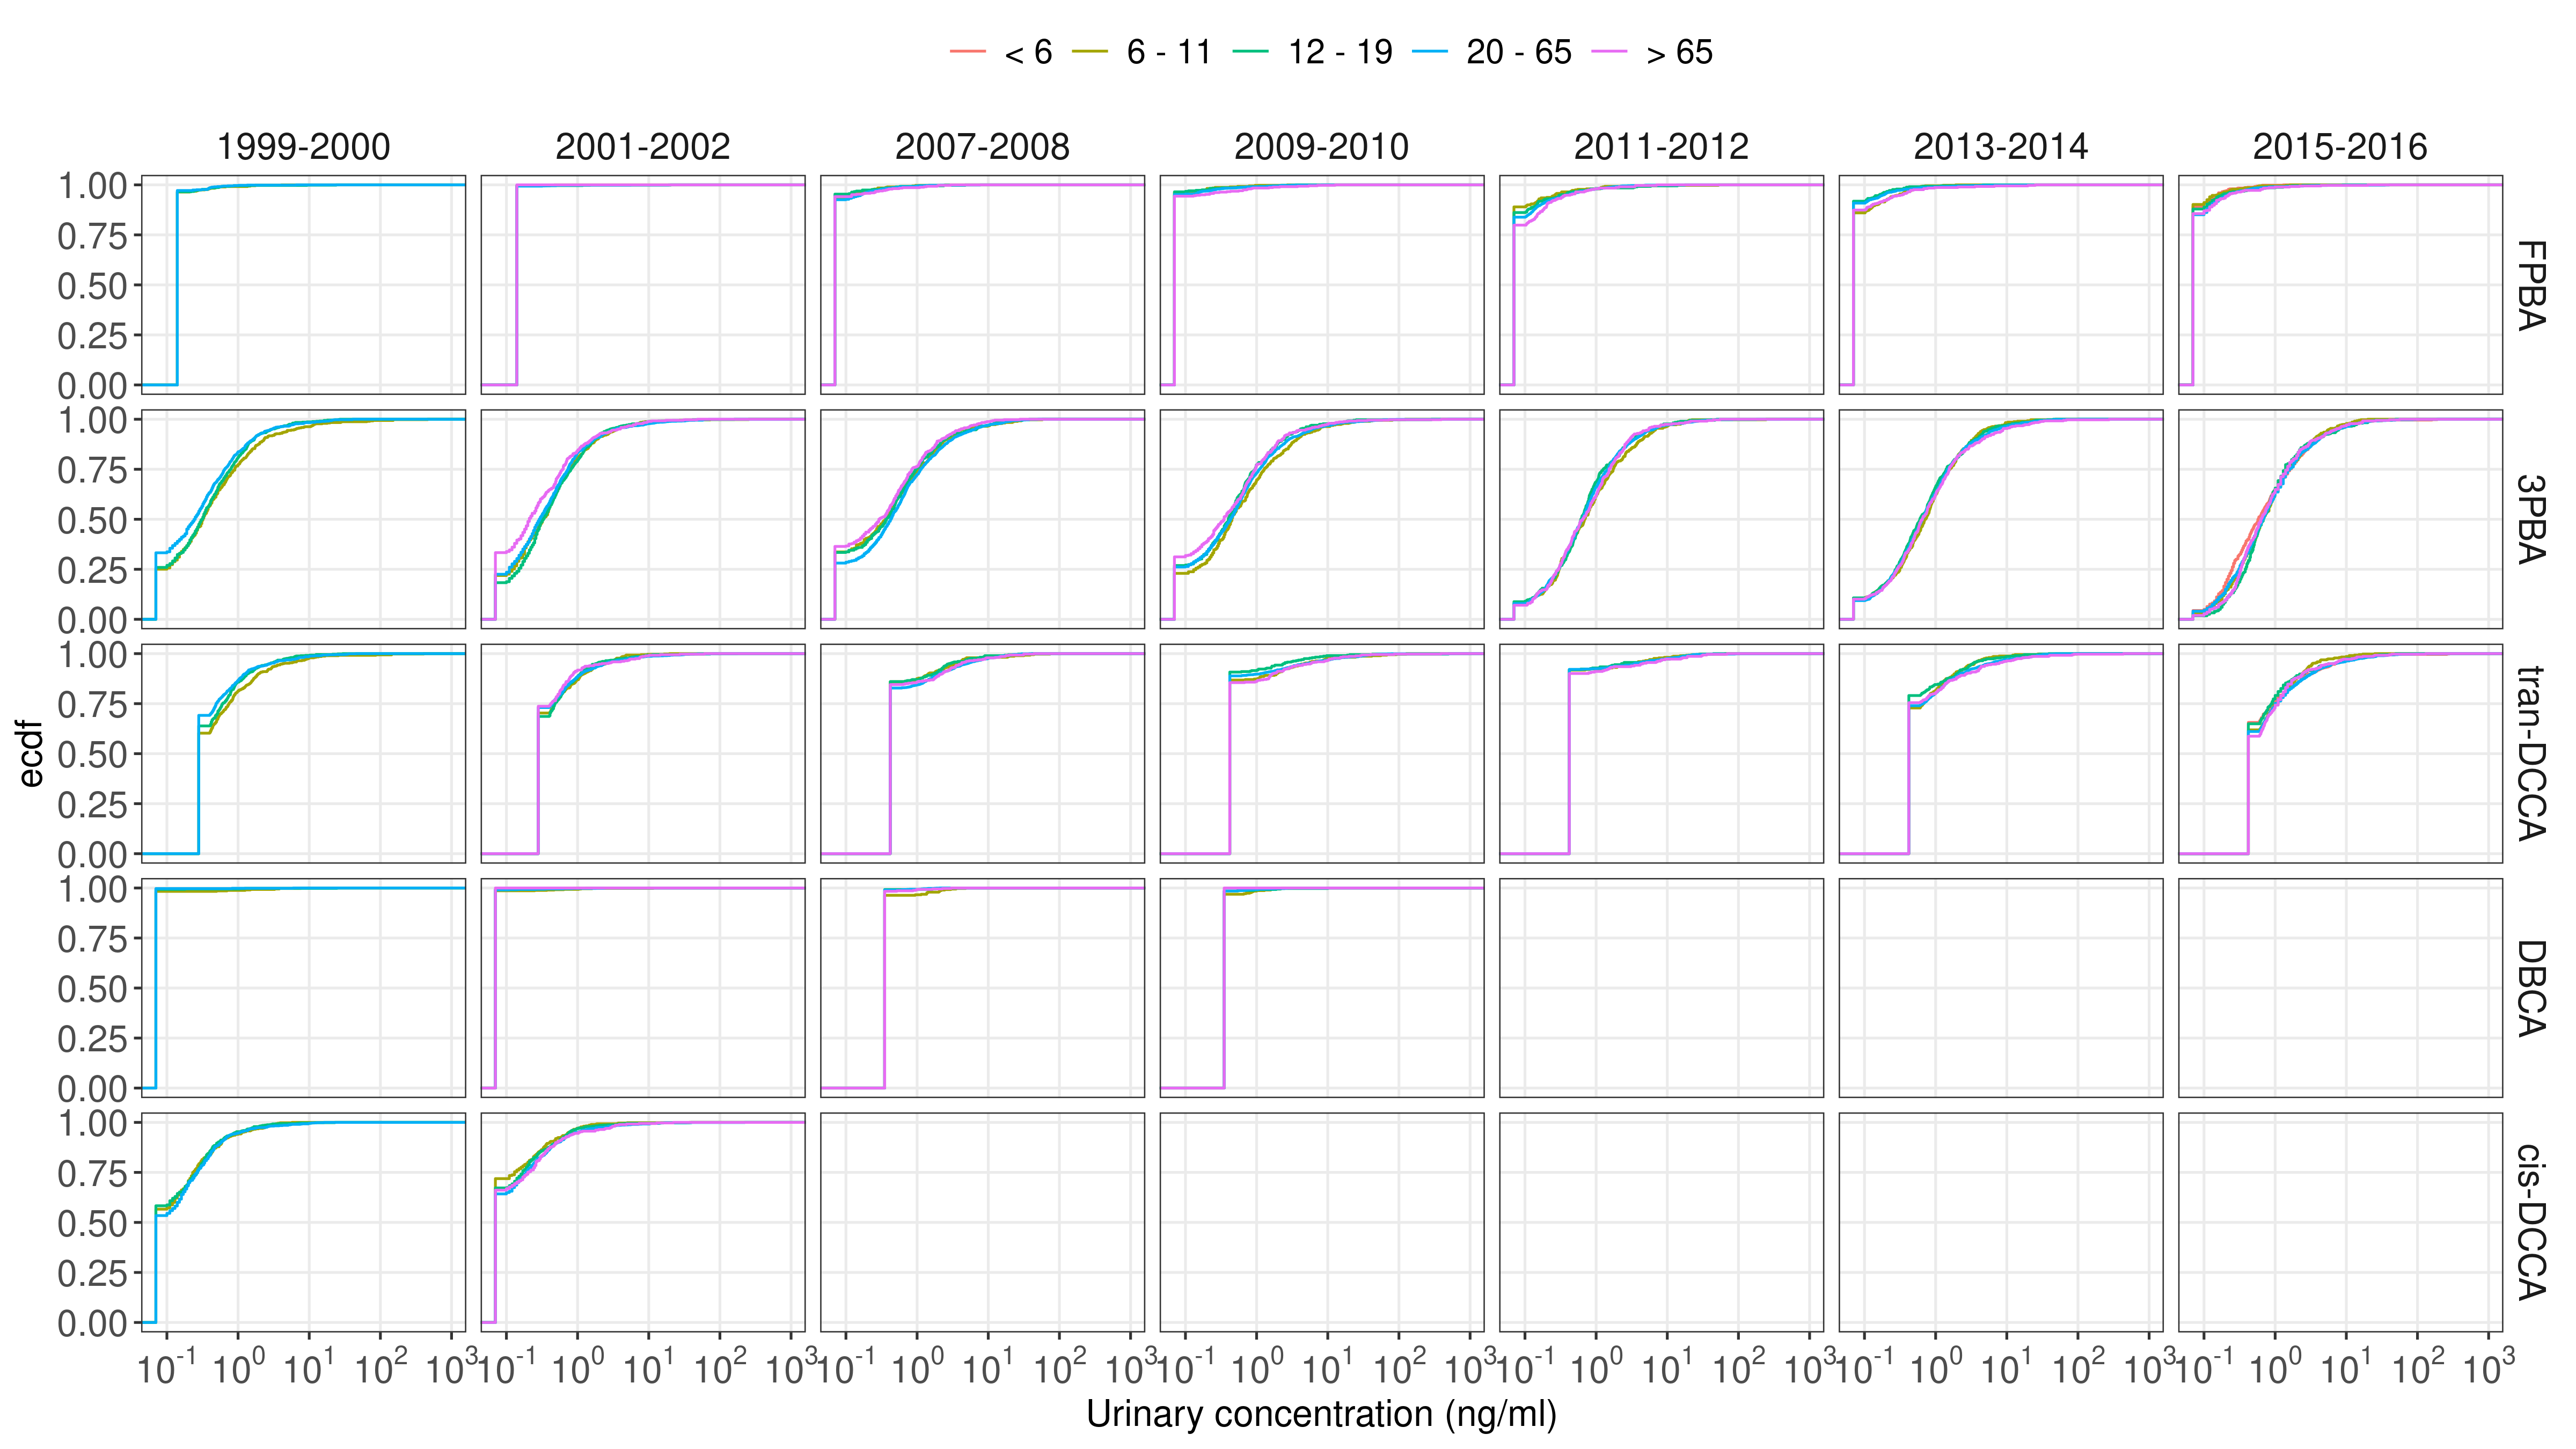
\includegraphics[width=\linewidth]{figures/figa1}
\hfill
\end{adjustwidth}
\caption{Cumulative distribution of urinary pyrethroid metabolite concentrations across different age groups.}\label{fig:figa1}
\end{figure}

\begin{figure}[H]
\begin{adjustwidth}{-4cm}{}
\includegraphics[width=\linewidth]{figures/figa2}
\hfill
\end{adjustwidth}
\caption{Evaluation of model performance of refined PBK model with human toxicokinetic experiments.}\label{fig:figa2}
\end{figure}


%%%%%%%%%%%%%%%%%%%%%%%%%%%%%%%%%%%%%%%%%%
%\isPreprints{} % If the paper is ``preprints'', please uncomment this parenthesis.
%\printendnotes[custom] % Un-comment to print a list of endnotes

\reftitle{References}

% Please provide either the correct journal abbreviation (e.g. according to the “List of Title Word Abbreviations” http://www.issn.org/services/online-services/access-to-the-ltwa/) or the full name of the journal.
% Citations and References in Supplementary files are permitted provided that they also appear in the reference list here. 

%=====================================
% References, variant A: external bibliography
%=====================================
\bibliography{references.bib}

% If authors have biography, please use the format below
%\section*{Short Biography of Authors}
%\bio
%{\raisebox{-0.35cm}{\includegraphics[width=3.5cm,height=5.3cm,clip,keepaspectratio]{Definitions/author1.pdf}}}
%{\textbf{Firstname Lastname} Biography of first author}
%
%\bio
%{\raisebox{-0.35cm}{\includegraphics[width=3.5cm,height=5.3cm,clip,keepaspectratio]{Definitions/author2.jpg}}}
%{\textbf{Firstname Lastname} Biography of second author}

% For the MDPI journals use author-date citation, please follow the formatting guidelines on http://www.mdpi.com/authors/references
% To cite two works by the same author: \citeauthor{ref-journal-1a} (\citeyear{ref-journal-1a}, \citeyear{ref-journal-1b}). This produces: Whittaker (1967, 1975)
% To cite two works by the same author with specific pages: \citeauthor{ref-journal-3a} (\citeyear{ref-journal-3a}, p. 328; \citeyear{ref-journal-3b}, p.475). This produces: Wong (1999, p. 328; 2000, p. 475)

%%%%%%%%%%%%%%%%%%%%%%%%%%%%%%%%%%%%%%%%%%
%% for journal Sci
%\reviewreports{\\
%Reviewer 1 comments and authors’ response\\
%Reviewer 2 comments and authors’ response\\
%Reviewer 3 comments and authors’ response
%}
%%%%%%%%%%%%%%%%%%%%%%%%%%%%%%%%%%%%%%%%%%
\PublishersNote{}
%\isPreprints{} % If the paper is ``preprints'', please uncomment this parenthesis.
\end{document}

